% Final version, generated from data/cbdc_corpus.csv by scripts/make_slides.py.
\PassOptionsToPackage{table}{xcolor}
\documentclass[aspectratio=169,10pt]{beamer}
\usetheme[progressbar=frametitle,sectionpage=progressbar]{metropolis}
\usepackage[utf8]{inputenc}
\usepackage[T1]{fontenc}
\usepackage{amsmath,amssymb,booktabs,pgfplots,listings,textcomp,nicefrac}
\usetikzlibrary{positioning,arrows.meta}
\pgfplotsset{compat=1.18}
\definecolor{c1}{HTML}{23395B}\definecolor{c2}{HTML}{D1495B}\definecolor{c3}{HTML}{EDAE49}
\definecolor{c4}{HTML}{00798C}\definecolor{c5}{HTML}{8F6593}\definecolor{c6}{HTML}{6A994E}
\definecolor{c7}{HTML}{E07A5F}\definecolor{c8}{HTML}{3D5A80}\definecolor{codebg}{HTML}{F3F3F0}
\pgfplotscreateplotcyclelist{corpus}{{fill=c1,draw=c1},{fill=c2,draw=c2},{fill=c3,draw=c3},{fill=c4,draw=c4}}
\lstset{language=Python, basicstyle=\ttfamily\fontsize{6.6}{7.6}\selectfont, keywordstyle=\color{c1}\bfseries,
  stringstyle=\color{c4}, backgroundcolor=\color{codebg}, frame=none, showstringspaces=false,
  columns=fullflexible, keepspaces=true, xleftmargin=4pt, framexleftmargin=4pt,
  upquote=true, literate={é}{{\'e}}1 {è}{{\`e}}1 {’}{{\textquotesingle}}1}
\tikzset{box/.style={draw=c1, rounded corners=2pt, fill=white, align=center, font=\scriptsize, minimum height=7mm,
  text width=19mm}, arr/.style={-{Stealth[length=2mm]}, c1, thick}}
\setbeamertemplate{note page}{\pagecolor{white}\vspace{6mm}\hspace{6mm}\begin{minipage}{0.9\paperwidth}\large\insertnote\end{minipage}}
\newcommand{\ymaxev}{51}

% links between each result and the slide that explains its method
\makeatletter\newcommand{\slabel}[1]{\edef\@currentlabel{\the\c@framenumber}\label{#1}}\makeatother
\newcommand{\method}[1]{\hfill\hyperref[#1]{\tiny\textcolor{c4}{$\triangleright$ method explained: slide~\ref*{#1}}}}
\newcommand{\usedon}[1]{\hyperref[#1]{\textcolor{c4}{slide~\ref*{#1}}}}
\newcommand{\mhead}[1]{\textcolor{c1}{\textbf{#1}}\\[1pt]}

\title{How Economists Discuss Central Bank Digital Currencies}
\subtitle{Themes, tone and stance, 2014--2026: a bibliometric and text-as-data study}
\author{Louis Drogo, Kenza Redwane and Adriel Mazere}
\institute{M2 -- Private crypto}
\date{October 2026}
\begin{document}
\begin{frame}
\titlepage
\note{\textbf{Title (0:15). Total: about 25 minutes.}}
\end{frame}

\begin{frame}{The paper in one slide}
\textbf{Research question.} How has economists and institutional discourse on CBDCs evolved between 2014 and 2026, and to what extent does this evolution align with changes in the policy environment?\\[5pt]
\small
\begin{tabular}{@{}ll@{}}
\alert{Who} writes? & research economists, central banks and institutions\\
\alert{What} do they write about? & themes and topics, and how they shift\\
\alert{How} do they discuss CBDCs? & \textbf{tone and stance: the core of the paper}\\
\alert{Why}, in their own words? & stated motivations\\
\alert{When}, and with which environment? & bursts, policy events, sanctions\\
\end{tabular}\\[5pt]
\textbf{Scope.} Descriptive: we measure changes and show what moves with them; we do not claim causes.
\vfill
\begin{center}48,188 texts collected \;$\to$\; 17,709 with CBDC as a theme \;$\to$\; \alert{4,710 written by economists}\end{center}
\note{\textbf{The paper in one slide (1:00).} One question, five sub-questions; tone and stance are the core.}
\end{frame}

\begin{frame}{Outline}
\tableofcontents
\note{\textbf{Outline (0:10).}}
\end{frame}

% =====================================================================
\section{Introduction}

\begin{frame}{Related literature: CBDCs}
% to be completed from the reading list
\note{\textbf{Literature (0:45).}}
\end{frame}

\begin{frame}{Related literature: what the field builds on}
% to be completed: reading list + co-citation clusters (section ``Who writes'')
\note{\textbf{Literature (0:45).}}
\end{frame}

\begin{frame}{What this paper adds to 29 earlier reviews}
\footnotesize Five recent bibliometric reviews:\\[2pt]
\begin{tabular}{@{}llrl@{}}\toprule
\textbf{Study} & \textbf{Data} & \textbf{Documents} & \textbf{Tools}\\\midrule
Kvedaravi\v{c}i\={u}t\.{e} \& \v{S}apkauskien\.{e} (2024) & WoS + Scopus & 228 & VOSviewer\\
Fahad \& Bulut (2024) & Scopus & 169 of 323 & Biblioshiny\\
Bapat \& Sharma (2025) & Scopus & 371 & bibliometrics + TCCM\\
Prodan et al.\ (2024) & Scopus + WoS & 747 of 1{,}024 & PRISMA, VOSviewer\\
Paulovici (2026) & Scopus & 892 & VOSviewer\\\midrule
\textbf{This study} & \textbf{5 databases + central banks} & \textbf{4,710} & \textbf{+ text as data}\\
\bottomrule\end{tabular}\\[6pt]
\small
\begin{itemize}\setlength\itemsep{1pt}
\item \alert{Gap}: one or two databases, mostly English journal articles; central banks absent; who writes is not checked.
\item Maps say \emph{what} is studied, not \emph{how} (tone, stance) or \emph{why}; no measure is validated.
\item \alert{Here}: economists only (checked text by text), all languages, tone and stance over time, every coder validated.
\end{itemize}
\scriptsize Found in our own corpus: 29 titles announce a literature, systematic or bibliometric review of CBDCs (2019--2026).
\note{\textbf{What this paper adds (1:00).} The closest is Hoang et al.\ (2023, RIBAF): text mining, but academic only and no stance.}
\end{frame}

\begin{frame}{Approach: one tool per question}
\scriptsize
\setlength{\tabcolsep}{4pt}
\begin{tabular}{@{}lp{0.36\textwidth}p{0.3\textwidth}l@{}}\toprule
\textbf{Question} & \textbf{Tool} & \textbf{Why this one} & \textbf{Explained}\\\midrule
Who? & co-citation, co-authorship (association strength, Louvain); laws; log-odds with Dirichlet prior & standard science maps; log-odds shrinks rare words & \usedon{m:net}, \usedon{m:logodds}\\
What? & thematic map; \alert{BERTopic} (SBERT, UMAP, HDBSCAN); labels by \alert{c-TF-IDF} & groups texts by meaning, across languages & \usedon{m:sbert}, \usedon{m:bertopic}\\
How? & tone: \alert{FinBERT} on CBDC sentences ($\kappa = 0.52$); stance: reading + \alert{local LLM} ($\kappa = 0.45$) & best of the coders tested against reading & \usedon{m:finbert}, \usedon{m:stance}\\
Why? & \alert{validated codebook} ($\kappa = 0.46$) + \alert{covariate logit} & beats SBERT, NLI, LLMs ($\kappa \le 0.25$) & \usedon{m:codebook}, \usedon{m:logit}\\
When? & \alert{Kleinberg bursts}; \alert{event studies} with placebo dates; \alert{difference-in-differences} & placebo fixes false positives (13\%) & \usedon{m:burst}, \usedon{m:event}, \usedon{m:did}\\\midrule
All & 7 robustness specifications; every coder checked on hand-coded texts & & \usedon{m:robust}\\
\bottomrule\end{tabular}\\[4pt]
\small Every result slide links to the slide that explains its method (appendix).
\note{\textbf{Approach (0:45).}}
\end{frame}

% =====================================================================
\section{Data}

\begin{frame}{Pipeline}
\begin{center}
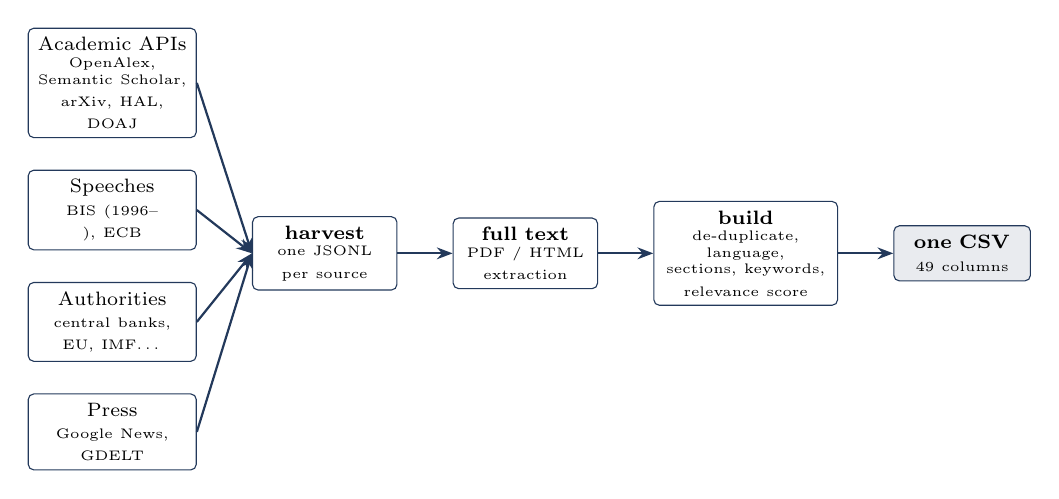
\begin{tikzpicture}[node distance=4mm and 7mm]
\node[box] (s1) {Academic APIs\\\tiny OpenAlex, Semantic Scholar,\\\tiny arXiv, HAL, DOAJ};
\node[box, below=of s1] (s2) {Speeches\\\tiny BIS (1996--), ECB};
\node[box, below=of s2] (s3) {Authorities\\\tiny central banks, EU, IMF\dots};
\node[box, below=of s3] (s4) {Press\\\tiny Google News, GDELT};
\node[box, right=of s2, yshift=-5.5mm, text width=16mm] (raw) {\textbf{harvest}\\\tiny one JSONL\\\tiny per source};
\node[box, right=of raw, text width=16mm] (ft) {\textbf{full text}\\\tiny PDF / HTML\\\tiny extraction};
\node[box, right=of ft, text width=21mm] (bd) {\textbf{build}\\\tiny de-duplicate, language,\\\tiny sections, keywords,\\\tiny relevance score};
\node[box, right=of bd, text width=15mm, fill=c1!10] (csv) {\textbf{one CSV}\\\tiny 49 columns};
\foreach \s in {s1,s2,s3,s4} \draw[arr] (\s.east) -- (raw.west);
\draw[arr] (raw) -- (ft); \draw[arr] (ft) -- (bd); \draw[arr] (bd) -- (csv);
\end{tikzpicture}
\end{center}
\small
\begin{itemize}
\item 115 search phrases, 12 languages: \emph{CBDC, digital euro, e-CNY, eNaira, Drex, digital fiat currency, Fedcoin, euro numérique, digitaler Euro, digital ruble\dots}
\item \alert{Recall first}: collect everything, then filter in four steps: homonyms, centrality, labels, \alert{economists}.
\end{itemize}
\note{\textbf{Pipeline (0:40).}}
\end{frame}

\begin{frame}[fragile]{Step 1: is it really \emph{Central Bank Digital Currency}?}
\begin{columns}[T]
\begin{column}{0.5\textwidth}
\begin{lstlisting}
TERMS = {
  "CBDC": r"\bCBDCs?\b|\bwCBDCs?\b|\brCBDCs?\b",
  "central bank digital currency":
      r"central[\s-]+banks?(?:['’]s?)?[\s-]+"
      r"digital[\s-]+currenc(?:y|ies)",
  "digital euro": r"digital(?:e[rn]?)?\s+euro\b"
      r"|euro\s+numérique|euro\s+digitale?\b",
  "DCEP (e-CNY)": r"\bDC/?EP\b",
  ...
}
\end{lstlisting}
\end{column}
\begin{column}{0.47\textwidth}\small
\begin{itemize}
\item ``CBDC'' is also a \emph{skin disease}; ``DCEP'' a chemical.
\item Ambiguous terms $t\in\mathcal{A}$ count only with \alert{monetary context}:
\end{itemize}
\[
\text{count}(t) = n_t \cdot \mathbf{1}\big[t \notin \mathcal{A} \,\lor\, \text{context}\big]
\]
\begin{itemize}
\item context = \emph{currency, payment, central bank, monnaie, Geld\dots}
\item \emph{digital dollar}, \emph{Sand Dollar}: reported, never scored.
\end{itemize}
\end{column}
\end{columns}
\note{\textbf{Homonyms (0:30).}}
\end{frame}

\begin{frame}{Step 2: how central is CBDC to the text?}
Each available field $f$ gets a centrality $c_f \in [0,1]$:
\begin{align*}
c_{\text{title}} &= \mathbf{1}[\text{CBDC term in title}] &
c_{\text{kw}} &= 0.4\cdot\mathbf{1}[\text{CBDC in keywords}]\\
c_{\text{abs}} &= \frac{\#\{\text{sentences mentioning CBDC}\}}{\#\{\text{sentences}\}} &
c_{\text{body}} &= \tfrac12\min\!\Big(1,\frac{\rho}{3}\Big) + \tfrac12\,\sigma
\end{align*}
$\rho$ = mentions per 1{,}000 words; $\sigma$ = share of the ten slices of the text that mention CBDC.
\[
\boxed{\text{score} = 100\Big(0.6\,\max_{f\in F} c_f + 0.4\,\frac{1}{|F|}\sum_{f\in F} c_f\Big)}
\qquad F = \text{fields available}
\]
\small One field clearly about CBDC suffices; a passing mention stays low; missing fields are not penalised.
\note{\textbf{Theme score (0:30).}}
\end{frame}

\begin{frame}{Step 3: labels, and how good is the filter?}
\begin{columns}[T]
\begin{column}{0.58\textwidth}\scriptsize
\setlength{\tabcolsep}{3pt}
\begin{tabular}{@{}lrrr@{}}\toprule
\textbf{Label (all texts kept)} & \textbf{Texts} & \textbf{Theme} & \textbf{95\% CI}\\\midrule
Main theme ($\geq 50$) & 15,464 & 29/30 & 0.83--0.99 \\
Secondary theme (25--49) & 2,245 & 11/29 & 0.23--0.56 \\
Mentioned only ($<25$) & 489 & 1/30 & 0.01--0.17 \\
Press, text not available & 13,446 & 2/19 & 0.03--0.31 \\
Ambiguous terms only & 1,709 & 3/10 & 0.11--0.60 \\
Off-topic (homonyms, no match) & 14,803 & 0/20 & 0.00--0.16 \\
Dated before 2014 (checked: false) & 32 & -- & -- \\
\bottomrule\end{tabular}\\[3pt]
Theme = share read as having CBDC as a theme, in a stratified sample of 138 texts read blind to the label; Wilson intervals.
\end{column}
\begin{column}{0.4\textwidth}\small
Strata $h$ weighted by size $N_h$; $T$ = theme labels:
\[ \widehat{P} = \frac{\sum_{h\in T} N_h \hat p_h}{\sum_{h\in T} N_h}, \qquad \widehat{R} = \frac{\sum_{h\in T} N_h \hat p_h}{\sum_{h} N_h \hat p_h} \]
\begin{itemize}\setlength\itemsep{1pt}
\item Precision \alert{0.89}, recall \alert{0.89}.
\item Secondary theme is noisy $\Rightarrow$ robustness on main theme only.
\end{itemize}
\end{column}
\end{columns}
\vspace{2pt}
\small Kept: \alert{main + secondary theme} (17,709 texts).
\note{\textbf{Validating the filter (0:40).}}
\end{frame}

\begin{frame}{Step 4: is it written by an economist?}
\slabel{r:econ}
\footnotesize
\begin{tabular}{@{}p{0.62\textwidth}rl@{}}\toprule
\textbf{Texts with CBDC as a theme} & \textbf{Texts} & \\\midrule
Research, classified in economics or finance (OpenAlex) & 3,783 & kept \\
Research, other field but an author at a central bank, IMF or BIS & 148 & kept \\
Research without OpenAlex record, economics venue & 63 & kept \\
Research in other fields & 3,469 & dropped \\
Central bank speeches & 511 & kept \\
Documents of central banks and international institutions & 205 & kept \\
Documents of governments and parliaments & 34 & dropped \\
Press articles (no author) & 9,496 & dropped \\
\bottomrule\end{tabular}\\[4pt]
\scriptsize Field = OpenAlex primary topic (``Economics, Econometrics and Finance''); institutions = authors' affiliations in OpenAlex. Research dropped: Computer Science 1,769, Business, Management and Accounting 663, no OpenAlex record 473, Social Sciences 281.\\[4pt]
\small
\begin{itemize}\setlength\itemsep{1pt}
\item \alert{4,710 texts by economists}: research economists, and central banks and international institutions (staff economists, institutional voice).
\item Press dropped: no author is known, and journalists are not economists.
\end{itemize}
\method{m:econ}
\note{\textbf{Economists (0:50).} This answers the course's question: the corpus is economists' writing, checked text by text.}
\end{frame}

\begin{frame}{Sources and completeness (economists' corpus)}
\begin{columns}[T]
\begin{column}{0.46\textwidth}\footnotesize
\begin{tabular}{@{}lr@{}}\toprule
\textbf{Database} & \textbf{Documents}\\\midrule
OpenAlex & 4,043 \\
Semantic Scholar & 2,164 \\
BIS central bankers' speeches & 465 \\
DOAJ & 251 \\
Central banks \& authorities (crawl) & 205 \\
ECB speeches & 108 \\
HAL & 31 \\
arXiv & 24 \\
\bottomrule\end{tabular}\\[2pt]
\scriptsize Merged duplicates count in each database.
\end{column}
\begin{column}{0.5\textwidth}\footnotesize
\begin{tabular}{@{}lr@{}}\toprule
\textbf{Type of text} & \textbf{Documents}\\\midrule
Academic & 3,994 \\
Speeches & 511 \\
Official docs & 205 \\
\midrule Total & 4,710\\\bottomrule\end{tabular}\\[6pt]
\begin{tabular}{@{}lr@{}}\toprule
\textbf{Field available} & \textbf{Share}\\\midrule
Exact day of publication & 71\% \\
Issuer / outlet identified & 97\% \\
Abstract & 68\% \\
Full text & 63\% \\
Keywords & 85\% \\
Reference list & 32\% \\
\bottomrule\end{tabular}
\end{column}
\end{columns}
\note{\textbf{Sources (0:30).}}
\end{frame}

\begin{frame}{A literature that took off after 2020}
\slabel{r:growth}
\begin{columns}[c]
\begin{column}{0.66\textwidth}
\begin{tikzpicture}
\begin{axis}[ybar stacked, width=\textwidth, height=0.7\textheight, bar width=11pt,
  cycle list name=corpus, xtick=data, xticklabel style={/pgf/number format/1000 sep=, font=\scriptsize, rotate=45, anchor=north east},
  ymin=0, legend style={at={(0.02,0.98)},anchor=north west,font=\scriptsize,draw=none},
  ylabel={Documents}, tick label style={font=\scriptsize}, axis lines*=left, ymajorgrids]
\addplot coordinates {(2016,3) (2017,20) (2018,36) (2019,77) (2020,161) (2021,284) (2022,315) (2023,572) (2024,623) (2025,839) (2026,898)};
\addlegendentry{Academic}
\addplot coordinates {(2016,3) (2017,8) (2018,30) (2019,24) (2020,41) (2021,66) (2022,77) (2023,67) (2024,67) (2025,72) (2026,56)};
\addlegendentry{Speeches}
\addplot coordinates {(2016,1) (2017,5) (2018,2) (2019,2) (2020,9) (2021,7) (2022,12) (2023,49) (2024,30) (2025,45) (2026,42)};
\addlegendentry{Official docs}
\end{axis}
\end{tikzpicture}
\end{column}
\begin{column}{0.32\textwidth}\small
\begin{itemize}
\item From 103 in 2019 to 956 in 2025.
\item Growth 60\% a year.
\item Turning point 2020: Libra (2019), COVID, the ECB report (Oct.\ 2020).
\end{itemize}
\scriptsize 0 documents before 2016; 2026 runs to October.
\end{column}
\end{columns}
\note{\textbf{Growth (0:30).}}
\end{frame}

\begin{frame}{Languages}
\begin{columns}[c]
\begin{column}{0.58\textwidth}
\begin{tikzpicture}
\begin{axis}[xbar, width=\textwidth, height=0.72\textheight, bar width=7pt, xmin=0,
  symbolic y coords={{Arabic},{Turkish},{Japanese},{Italian},{Portuguese},{French},{Spanish},{Ukrainian},{German},{Russian}}, ytick=data, tick label style={font=\scriptsize},
  axis lines*=left, nodes near coords, nodes near coords style={font=\tiny},
  xlabel={Documents}, xlabel style={font=\scriptsize}, enlarge x limits={upper,value=0.12}]
\addplot[fill=c1, draw=c1] coordinates {(12,{Arabic}) (24,{Turkish}) (26,{Japanese}) (28,{Italian}) (31,{Portuguese}) (43,{French}) (74,{Spanish}) (91,{Ukrainian}) (94,{German}) (422,{Russian})};
\end{axis}
\end{tikzpicture}
\end{column}
\begin{column}{0.4\textwidth}\small
\begin{itemize}
\item English dominates: 3,721 texts (79\%); the chart shows the others.
\item Second language: \alert{Russian} (422 texts).
\item Everything kept in its original language: the topic model and the codebook are multilingual.
\end{itemize}
\end{column}
\end{columns}
\note{\textbf{Languages (0:20).}}
\end{frame}

% =====================================================================
\section{Who writes}

\begin{frame}{Research economists: outlets, most cited, laws}
\slabel{r:research}
\begin{columns}[T]
\begin{column}{0.4\textwidth}\scriptsize\textbf{Main outlets}\\[2pt]
\begin{tabular}{@{}p{0.8\linewidth}r@{}}SSRN Electronic Journal & 461 \\
RePEc: Research Papers in Economics & 164 \\
Zenodo (CERN repository) & 126 \\
CyberLeninka (Russian repository) & 70 \\
Springer eBooks & 68 \\
Routledge eBooks & 56 \\
Ekonomika i Upravlenie & 47 \\\end{tabular}\\[4pt]
\textbf{Bibliometric laws.} Growth 60\%/year (2017--2025). Lotka: $f(n) \propto n^{-3.3}$, 83\% of authors publish once. Bradford: 21 core sources hold \nicefrac{1}{3} of the papers (zones 21 : 310 : 1,148).
\end{column}
\begin{column}{0.58\textwidth}\scriptsize\textbf{Most cited papers} (global citations)\\[2pt]
\begin{tabular}{@{}p{0.2\linewidth}p{0.66\linewidth}r@{}}
Bordo (2017) & Central Bank Digital Currency and the Future of Monetary\dots{} & 517 \\
Auer (2020) & Rise of the Central Bank Digital Currencies: Drivers, App\dots{} & 454 \\
Agur (2019) & Designing Central Bank Digital Currencies & 433 \\
Andolfatto (2020) & Assessing the Impact of Central Bank Digital Currency on\dots{} & 404 \\
Barrdear (2016) & The Macroeconomics of Central Bank Issued Digital Currenc\dots{} & 341 \\
\end{tabular}\\[6pt]
\small Working papers (SSRN, RePEc) weigh as much as journals; a young, open field: most authors write once.
\end{column}
\end{columns}
\method{m:laws}
\note{\textbf{Research economists (0:40).}}
\end{frame}

\begin{frame}{Who speaks: central banks, institutions, research centres}
\begin{columns}[T]\begin{column}{0.32\textwidth}\scriptsize\textbf{Speeches, by central bank}\\[2pt]\begin{tabular}{@{}p{0.8\linewidth}r@{}}European Central Bank & 118 \\
Deutsche Bundesbank & 63 \\
Bank of France & 49 \\
Hong Kong Monetary Authority & 23 \\
Federal Reserve Board & 21 \\
Bank of England & 21 \\
Bank of Italy & 19 \\
Bank of Japan & 14 \\\end{tabular}\end{column}\begin{column}{0.32\textwidth}\scriptsize\textbf{Documents, by institution}\\[2pt]\begin{tabular}{@{}p{0.8\linewidth}r@{}}European Central Bank & 98 \\
Bank of Japan & 27 \\
Sveriges Riksbank & 22 \\
Deutsche Bundesbank & 21 \\
Swiss National Bank & 9 \\
Central Bank of The Bahamas & 7 \\
Bank of Jamaica & 6 \\
Bank of Canada & 4 \\\end{tabular}\end{column}\begin{column}{0.32\textwidth}\scriptsize\textbf{Research, by author institution}\\[2pt]\begin{tabular}{@{}p{0.8\linewidth}r@{}}Financial University & 63 \\
European Central Bank & 61 \\
International Monetary Fund & 39 \\
Bank of Canada & 38 \\
The Russian Presidential Acad\dots{} & 33 \\
Bank for International Settle\dots{} & 32 \\
Moscow State Institute of Int\dots{} & 29 \\
Lomonosov Moscow State Univer\dots{} & 29 \\\end{tabular}\end{column}\end{columns}
\vspace{3pt}
\small \alert{European Central Bank} is the most vocal central bank: the digital euro makes it the hub of the debate.
\note{\textbf{Voices (0:35).} Institutions under their own names: speeches by central bank, documents by institution, research by the authors' institutions.}
\end{frame}

\begin{frame}{Co-citation: the intellectual base}
\slabel{r:cocit}
\begin{columns}[T]
\begin{column}{0.7\textwidth}
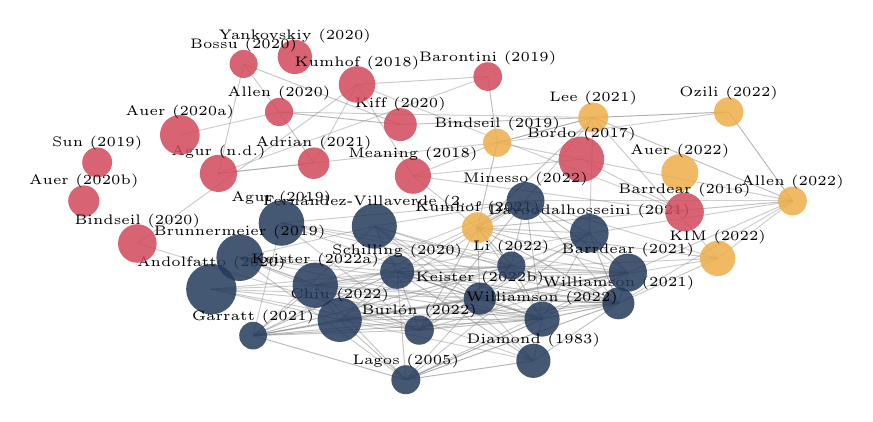
\begin{tikzpicture}
\draw[gray, opacity=0.67, line width=0.35pt] (6.47,3.33) -- (5.25,3.01);
\draw[gray, opacity=0.66, line width=0.35pt] (6.79,0.97) -- (5.03,1.03);
\draw[gray, opacity=0.66, line width=0.35pt] (4.09,0.00) -- (5.82,0.77);
\draw[gray, opacity=0.63, line width=0.35pt] (6.47,3.33) -- (8.19,3.40);
\draw[gray, opacity=0.63, line width=0.35pt] (6.79,0.97) -- (5.82,0.77);
\draw[gray, opacity=0.62, line width=0.35pt] (4.09,0.00) -- (6.79,0.97);
\draw[gray, opacity=0.60, line width=0.35pt] (5.82,0.77) -- (3.98,1.37);
\draw[gray, opacity=0.59, line width=0.35pt] (5.00,1.93) -- (5.43,1.45);
\draw[gray, opacity=0.58, line width=0.35pt] (5.43,1.45) -- (4.26,0.63);
\draw[gray, opacity=0.58, line width=0.35pt] (4.02,3.24) -- (2.48,3.40);
\draw[gray, opacity=0.58, line width=0.35pt] (4.09,0.00) -- (5.71,0.24);
\draw[gray, opacity=0.57, line width=0.35pt] (9.00,2.27) -- (8.19,3.40);
\draw[gray, opacity=0.56, line width=0.35pt] (6.79,0.97) -- (3.98,1.37);
\draw[gray, opacity=0.55, line width=0.35pt] (5.00,1.93) -- (6.79,0.97);
\draw[gray, opacity=0.55, line width=0.35pt] (5.03,1.03) -- (3.98,1.37);
\draw[gray, opacity=0.55, line width=0.35pt] (5.03,1.03) -- (5.82,0.77);
\draw[gray, opacity=0.55, line width=0.35pt] (4.09,0.00) -- (2.15,0.56);
\draw[gray, opacity=0.54, line width=0.35pt] (5.82,0.77) -- (5.43,1.45);
\draw[gray, opacity=0.54, line width=0.35pt] (6.79,0.97) -- (6.42,1.86);
\draw[gray, opacity=0.54, line width=0.35pt] (5.00,1.93) -- (5.03,1.03);
\draw[gray, opacity=0.54, line width=0.35pt] (5.82,0.77) -- (2.15,0.56);
\draw[gray, opacity=0.54, line width=0.35pt] (3.98,1.37) -- (2.15,0.56);
\draw[gray, opacity=0.52, line width=0.35pt] (5.61,2.27) -- (6.91,1.36);
\draw[gray, opacity=0.52, line width=0.35pt] (5.43,1.45) -- (2.15,0.56);
\draw[gray, opacity=0.52, line width=0.35pt] (5.25,3.01) -- (5.13,3.85);
\draw[gray, opacity=0.51, line width=0.35pt] (5.00,1.93) -- (5.25,3.01);
\draw[gray, opacity=0.51, line width=0.35pt] (6.42,1.86) -- (6.91,1.36);
\draw[gray, opacity=0.51, line width=0.35pt] (3.98,1.37) -- (5.71,0.24);
\draw[gray, opacity=0.51, line width=0.35pt] (5.82,0.77) -- (4.26,0.63);
\draw[gray, opacity=0.50, line width=0.35pt] (6.47,3.33) -- (4.02,3.24);
\draw[gray, opacity=0.50, line width=0.35pt] (6.79,0.97) -- (6.91,1.36);
\draw[gray, opacity=0.50, line width=0.35pt] (6.79,0.97) -- (5.43,1.45);
\draw[gray, opacity=0.50, line width=0.35pt] (6.47,3.33) -- (9.00,2.27);
\draw[gray, opacity=0.49, line width=0.35pt] (3.25,0.76) -- (2.15,0.56);
\draw[gray, opacity=0.49, line width=0.35pt] (5.82,0.77) -- (2.94,1.20);
\draw[gray, opacity=0.49, line width=0.35pt] (6.79,0.97) -- (2.15,0.56);
\draw[gray, opacity=0.49, line width=0.35pt] (5.00,1.93) -- (4.26,0.63);
\draw[gray, opacity=0.49, line width=0.35pt] (6.47,3.33) -- (5.00,1.93);
\draw[gray, opacity=0.49, line width=0.35pt] (5.61,2.27) -- (4.26,0.63);
\draw[gray, opacity=0.49, line width=0.35pt] (4.09,0.00) -- (3.25,0.76);
\draw[gray, opacity=0.49, line width=0.35pt] (9.00,2.27) -- (5.00,1.93);
\draw[gray, opacity=0.49, line width=0.35pt] (3.25,0.76) -- (5.82,0.77);
\draw[gray, opacity=0.48, line width=0.35pt] (3.98,1.37) -- (4.26,0.63);
\draw[gray, opacity=0.48, line width=0.35pt] (5.00,1.93) -- (8.05,1.54);
\draw[gray, opacity=0.48, line width=0.35pt] (6.79,0.97) -- (5.71,0.24);
\draw[gray, opacity=0.48, line width=0.35pt] (6.42,1.86) -- (5.61,2.27);
\draw[gray, opacity=0.47, line width=0.35pt] (4.09,0.00) -- (3.98,1.37);
\draw[gray, opacity=0.47, line width=0.35pt] (5.82,0.77) -- (6.91,1.36);
\draw[gray, opacity=0.47, line width=0.35pt] (5.03,1.03) -- (5.43,1.45);
\draw[gray, opacity=0.47, line width=0.35pt] (5.00,1.93) -- (5.61,2.27);
\draw[gray, opacity=0.47, line width=0.35pt] (3.69,1.95) -- (5.03,1.03);
\draw[gray, opacity=0.47, line width=0.35pt] (3.25,0.76) -- (3.98,1.37);
\draw[gray, opacity=0.47, line width=0.35pt] (5.61,2.27) -- (5.82,0.77);
\draw[gray, opacity=0.47, line width=0.35pt] (5.82,0.77) -- (5.71,0.24);
\draw[gray, opacity=0.46, line width=0.35pt] (3.69,1.95) -- (3.98,1.37);
\draw[gray, opacity=0.46, line width=0.35pt] (3.25,0.76) -- (2.94,1.20);
\draw[gray, opacity=0.46, line width=0.35pt] (5.61,2.27) -- (5.43,1.45);
\draw[gray, opacity=0.46, line width=0.35pt] (6.79,0.97) -- (3.69,1.95);
\draw[gray, opacity=0.46, line width=0.35pt] (2.15,0.56) -- (2.94,1.20);
\draw[gray, opacity=0.46, line width=0.35pt] (6.91,1.36) -- (4.26,0.63);
\draw[gray, opacity=0.46, line width=0.35pt] (3.25,0.76) -- (4.26,0.63);
\draw[gray, opacity=0.46, line width=0.35pt] (2.15,0.56) -- (6.91,1.36);
\draw[gray, opacity=0.46, line width=0.35pt] (4.02,3.24) -- (2.03,4.01);
\draw[gray, opacity=0.45, line width=0.35pt] (2.94,1.20) -- (4.26,0.63);
\draw[gray, opacity=0.45, line width=0.35pt] (5.61,2.27) -- (3.98,1.37);
\draw[gray, opacity=0.45, line width=0.35pt] (4.09,0.00) -- (2.94,1.20);
\draw[gray, opacity=0.45, line width=0.35pt] (2.48,3.40) -- (2.92,2.75);
\draw[gray, opacity=0.44, line width=0.35pt] (6.42,1.86) -- (5.82,0.77);
\draw[gray, opacity=0.44, line width=0.35pt] (4.09,0.00) -- (1.98,1.55);
\draw[gray, opacity=0.44, line width=0.35pt] (5.00,1.93) -- (6.91,1.36);
\draw[gray, opacity=0.44, line width=0.35pt] (2.15,0.56) -- (4.26,0.63);
\draw[gray, opacity=0.44, line width=0.35pt] (6.79,0.97) -- (5.61,2.27);
\draw[gray, opacity=0.43, line width=0.35pt] (5.03,1.03) -- (2.15,0.56);
\draw[gray, opacity=0.43, line width=0.35pt] (8.05,1.54) -- (6.79,0.97);
\draw[gray, opacity=0.43, line width=0.35pt] (1.62,1.15) -- (3.25,0.76);
\draw[gray, opacity=0.43, line width=0.35pt] (3.47,3.75) -- (5.13,3.85);
\draw[gray, opacity=0.43, line width=0.35pt] (5.00,1.93) -- (6.42,1.86);
\draw[gray, opacity=0.43, line width=0.35pt] (3.25,0.76) -- (5.43,1.45);
\draw[gray, opacity=0.43, line width=0.35pt] (5.03,1.03) -- (4.26,0.63);
\draw[gray, opacity=0.43, line width=0.35pt] (4.09,0.00) -- (6.91,1.36);
\draw[gray, opacity=0.43, line width=0.35pt] (3.25,0.76) -- (6.79,0.97);
\draw[gray, opacity=0.43, line width=0.35pt] (3.25,0.76) -- (5.03,1.03);
\draw[gray, opacity=0.43, line width=0.35pt] (3.98,1.37) -- (6.91,1.36);
\draw[gray, opacity=0.43, line width=0.35pt] (1.62,1.15) -- (5.82,0.77);
\draw[gray, opacity=0.43, line width=0.35pt] (5.03,1.03) -- (6.91,1.36);
\draw[gray, opacity=0.43, line width=0.35pt] (1.71,2.62) -- (2.03,4.01);
\draw[gray, opacity=0.43, line width=0.35pt] (3.98,1.37) -- (2.94,1.20);
\draw[gray, opacity=0.42, line width=0.35pt] (3.98,1.37) -- (1.98,1.55);
\draw[gray, opacity=0.42, line width=0.35pt] (5.43,1.45) -- (2.94,1.20);
\draw[gray, opacity=0.42, line width=0.35pt] (4.09,0.00) -- (6.42,1.86);
\draw[gray, opacity=0.42, line width=0.35pt] (3.47,3.75) -- (0.68,1.73);
\draw[gray, opacity=0.42, line width=0.35pt] (4.18,2.59) -- (3.47,3.75);
\draw[gray, opacity=0.42, line width=0.35pt] (4.09,0.00) -- (5.03,1.03);
\draw[gray, opacity=0.42, line width=0.35pt] (3.69,1.95) -- (2.15,0.56);
\draw[gray, opacity=0.42, line width=0.35pt] (6.79,0.97) -- (2.94,1.20);
\draw[gray, opacity=0.42, line width=0.35pt] (1.71,2.62) -- (2.92,2.75);
\draw[gray, opacity=0.42, line width=0.35pt] (5.82,0.77) -- (1.98,1.55);
\draw[gray, opacity=0.42, line width=0.35pt] (6.79,0.97) -- (4.26,0.63);
\draw[gray, opacity=0.42, line width=0.35pt] (6.42,1.86) -- (5.03,1.03);
\draw[gray, opacity=0.42, line width=0.35pt] (6.32,2.80) -- (7.63,2.13);
\draw[gray, opacity=0.42, line width=0.35pt] (1.62,1.15) -- (4.26,0.63);
\draw[gray, opacity=0.41, line width=0.35pt] (2.94,1.20) -- (6.91,1.36);
\draw[gray, opacity=0.41, line width=0.35pt] (4.18,2.59) -- (7.63,2.13);
\draw[gray, opacity=0.41, line width=0.35pt] (5.43,1.45) -- (6.91,1.36);
\draw[gray, opacity=0.41, line width=0.35pt] (5.61,2.27) -- (2.51,1.99);
\draw[gray, opacity=0.41, line width=0.35pt] (9.00,2.27) -- (6.42,1.86);
\draw[gray, opacity=0.41, line width=0.35pt] (9.00,2.27) -- (5.25,3.01);
\draw[gray, opacity=0.41, line width=0.35pt] (4.18,2.59) -- (5.25,3.01);
\draw[gray, opacity=0.41, line width=0.35pt] (6.47,3.33) -- (2.48,3.40);
\draw[gray, opacity=0.41, line width=0.35pt] (1.62,1.15) -- (3.98,1.37);
\draw[gray, opacity=0.41, line width=0.35pt] (6.47,3.33) -- (8.05,1.54);
\draw[gray, opacity=0.41, line width=0.35pt] (9.00,2.27) -- (6.91,1.36);
\draw[gray, opacity=0.41, line width=0.35pt] (1.98,1.55) -- (4.26,0.63);
\draw[gray, opacity=0.41, line width=0.35pt] (2.51,1.99) -- (6.91,1.36);
\draw[gray, opacity=0.41, line width=0.35pt] (6.47,3.33) -- (6.42,1.86);
\draw[gray, opacity=0.40, line width=0.35pt] (5.03,1.03) -- (2.94,1.20);
\draw[gray, opacity=0.40, line width=0.35pt] (3.25,0.76) -- (6.91,1.36);
\draw[gray, opacity=0.40, line width=0.35pt] (2.48,3.40) -- (2.03,4.01);
\draw[gray, opacity=0.40, line width=0.35pt] (4.18,2.59) -- (5.00,1.93);
\draw[gray, opacity=0.40, line width=0.35pt] (5.71,0.24) -- (1.98,1.55);
\draw[gray, opacity=0.40, line width=0.35pt] (4.26,0.63) -- (0.68,1.73);
\draw[gray, opacity=0.40, line width=0.35pt] (5.03,1.03) -- (5.71,0.24);
\draw[gray, opacity=0.40, line width=0.35pt] (6.79,0.97) -- (1.98,1.55);
\draw[gray, opacity=0.40, line width=0.35pt] (6.79,0.97) -- (2.51,1.99);
\draw[gray, opacity=0.40, line width=0.35pt] (5.00,1.93) -- (5.82,0.77);
\draw[gray, opacity=0.40, line width=0.35pt] (1.62,1.15) -- (2.94,1.20);
\draw[gray, opacity=0.40, line width=0.35pt] (3.69,1.95) -- (5.71,0.24);
\draw[gray, opacity=0.39, line width=0.35pt] (5.61,2.27) -- (2.94,1.20);
\draw[gray, opacity=0.39, line width=0.35pt] (3.69,1.95) -- (5.82,0.77);
\draw[gray, opacity=0.39, line width=0.35pt] (2.51,1.99) -- (4.26,0.63);
\draw[gray, opacity=0.39, line width=0.35pt] (8.05,1.54) -- (3.98,1.37);
\draw[gray, opacity=0.39, line width=0.35pt] (8.05,1.54) -- (5.61,2.27);
\draw[gray, opacity=0.39, line width=0.35pt] (5.25,3.01) -- (8.19,3.40);
\draw[gray, opacity=0.39, line width=0.35pt] (5.82,0.77) -- (2.51,1.99);
\draw[gray, opacity=0.39, line width=0.35pt] (3.69,1.95) -- (5.61,2.27);
\draw[gray, opacity=0.39, line width=0.35pt] (2.51,1.99) -- (2.15,0.56);
\draw[gray, opacity=0.39, line width=0.35pt] (9.00,2.27) -- (8.05,1.54);
\draw[gray, opacity=0.39, line width=0.35pt] (6.42,1.86) -- (5.43,1.45);
\draw[gray, opacity=0.39, line width=0.35pt] (3.47,3.75) -- (7.63,2.13);
\draw[gray, opacity=0.39, line width=0.35pt] (1.71,2.62) -- (5.13,3.85);
\draw[gray, opacity=0.39, line width=0.35pt] (3.69,1.95) -- (5.43,1.45);
\draw[gray, opacity=0.39, line width=0.35pt] (8.05,1.54) -- (5.03,1.03);
\draw[gray, opacity=0.39, line width=0.35pt] (1.71,2.62) -- (5.25,3.01);
\draw[gray, opacity=0.39, line width=0.35pt] (9.00,2.27) -- (6.79,0.97);
\draw[gray, opacity=0.39, line width=0.35pt] (3.25,0.76) -- (5.61,2.27);
\draw[gray, opacity=0.39, line width=0.35pt] (3.69,1.95) -- (1.98,1.55);
\draw[gray, opacity=0.39, line width=0.35pt] (1.98,1.55) -- (2.94,1.20);
\draw[gray, opacity=0.39, line width=0.35pt] (6.42,1.86) -- (4.26,0.63);
\draw[gray, opacity=0.39, line width=0.35pt] (2.48,3.40) -- (1.22,3.11);
\draw[gray, opacity=0.38, line width=0.35pt] (9.00,2.27) -- (5.61,2.27);
\draw[gray, opacity=0.38, line width=0.35pt] (1.62,1.15) -- (6.79,0.97);
\draw[gray, opacity=0.38, line width=0.35pt] (3.25,0.76) -- (5.71,0.24);
\draw[gray, opacity=0.38, line width=0.35pt] (5.61,2.27) -- (2.15,0.56);
\draw[gray, opacity=0.38, line width=0.35pt] (1.98,1.55) -- (6.91,1.36);
\draw[gray, opacity=0.38, line width=0.35pt] (6.42,1.86) -- (2.94,1.20);
\draw[gray, opacity=0.38, line width=0.35pt] (2.51,1.99) -- (5.43,1.45);
\draw[gray, opacity=0.38, line width=0.35pt] (3.47,3.75) -- (2.92,2.75);
\draw[gray, opacity=0.38, line width=0.35pt] (4.18,2.59) -- (6.32,2.80);
\draw[gray, opacity=0.38, line width=0.35pt] (3.98,1.37) -- (5.43,1.45);
\draw[gray, opacity=0.38, line width=0.35pt] (6.47,3.33) -- (5.61,2.27);
\fill[c2, opacity=0.85] (2.68,4.10) circle (2.18mm);
\node[font=\fontsize{4.6}{5}\selectfont, above=1.53mm, inner sep=0.5pt] at (2.68,4.10) {Yankovskiy (2020)};
\fill[c3, opacity=0.85] (6.47,3.33) circle (1.90mm);
\node[font=\fontsize{4.6}{5}\selectfont, above=1.33mm, inner sep=0.5pt] at (6.47,3.33) {Lee (2021)};
\fill[c3, opacity=0.85] (9.00,2.27) circle (1.83mm);
\node[font=\fontsize{4.6}{5}\selectfont, above=1.28mm, inner sep=0.5pt] at (9.00,2.27) {Allen (2022)};
\fill[c1, opacity=0.85] (1.62,1.15) circle (3.20mm);
\node[font=\fontsize{4.6}{5}\selectfont, above=2.24mm, inner sep=0.5pt] at (1.62,1.15) {Andolfatto (2020)};
\fill[c2, opacity=0.85] (4.02,3.24) circle (2.09mm);
\node[font=\fontsize{4.6}{5}\selectfont, above=1.46mm, inner sep=0.5pt] at (4.02,3.24) {Kiff (2020)};
\fill[c1, opacity=0.85] (4.09,0.00) circle (1.84mm);
\node[font=\fontsize{4.6}{5}\selectfont, above=1.29mm, inner sep=0.5pt] at (4.09,0.00) {Lagos (2005)};
\fill[c1, opacity=0.85] (3.25,0.76) circle (2.81mm);
\node[font=\fontsize{4.6}{5}\selectfont, above=1.97mm, inner sep=0.5pt] at (3.25,0.76) {Chiu (2022)};
\fill[c2, opacity=0.85] (4.18,2.59) circle (2.29mm);
\node[font=\fontsize{4.6}{5}\selectfont, above=1.61mm, inner sep=0.5pt] at (4.18,2.59) {Meaning (2018)};
\fill[c2, opacity=0.85] (1.71,2.62) circle (2.36mm);
\node[font=\fontsize{4.6}{5}\selectfont, above=1.65mm, inner sep=0.5pt] at (1.71,2.62) {Agur (n.d.)};
\fill[c2, opacity=0.85] (0.17,2.76) circle (1.90mm);
\node[font=\fontsize{4.6}{5}\selectfont, above=1.33mm, inner sep=0.5pt] at (0.17,2.76) {Sun (2019)};
\fill[c2, opacity=0.85] (3.47,3.75) circle (2.32mm);
\node[font=\fontsize{4.6}{5}\selectfont, above=1.63mm, inner sep=0.5pt] at (3.47,3.75) {Kumhof (2018)};
\fill[c3, opacity=0.85] (5.00,1.93) circle (1.97mm);
\node[font=\fontsize{4.6}{5}\selectfont, above=1.38mm, inner sep=0.5pt] at (5.00,1.93) {Kumhof (2021)};
\fill[c3, opacity=0.85] (7.57,2.63) circle (2.35mm);
\node[font=\fontsize{4.6}{5}\selectfont, above=1.64mm, inner sep=0.5pt] at (7.57,2.63) {Auer (2022)};
\fill[c3, opacity=0.85] (8.05,1.54) circle (2.24mm);
\node[font=\fontsize{4.6}{5}\selectfont, above=1.57mm, inner sep=0.5pt] at (8.05,1.54) {KIM (2022)};
\fill[c1, opacity=0.85] (6.79,0.97) circle (2.03mm);
\node[font=\fontsize{4.6}{5}\selectfont, above=1.42mm, inner sep=0.5pt] at (6.79,0.97) {Williamson (2021)};
\fill[c1, opacity=0.85] (6.42,1.86) circle (2.45mm);
\node[font=\fontsize{4.6}{5}\selectfont, above=1.72mm, inner sep=0.5pt] at (6.42,1.86) {Davoodalhosseini (2021)};
\fill[c2, opacity=0.85] (6.32,2.80) circle (2.89mm);
\node[font=\fontsize{4.6}{5}\selectfont, above=2.02mm, inner sep=0.5pt] at (6.32,2.80) {Bordo (2017)};
\fill[c1, opacity=0.85] (3.69,1.95) circle (2.86mm);
\node[font=\fontsize{4.6}{5}\selectfont, above=2.00mm, inner sep=0.5pt] at (3.69,1.95) {Fernández-Villaverde (2\dots{}};
\fill[c3, opacity=0.85] (5.25,3.01) circle (1.79mm);
\node[font=\fontsize{4.6}{5}\selectfont, above=1.25mm, inner sep=0.5pt] at (5.25,3.01) {Bindseil (2019)};
\fill[c1, opacity=0.85] (5.61,2.27) circle (2.41mm);
\node[font=\fontsize{4.6}{5}\selectfont, above=1.69mm, inner sep=0.5pt] at (5.61,2.27) {Minesso (2022)};
\fill[c3, opacity=0.85] (8.19,3.40) circle (1.87mm);
\node[font=\fontsize{4.6}{5}\selectfont, above=1.31mm, inner sep=0.5pt] at (8.19,3.40) {Ozili (2022)};
\fill[c1, opacity=0.85] (5.03,1.03) circle (2.05mm);
\node[font=\fontsize{4.6}{5}\selectfont, above=1.43mm, inner sep=0.5pt] at (5.03,1.03) {Keister (2022b)};
\fill[c1, opacity=0.85] (5.82,0.77) circle (2.23mm);
\node[font=\fontsize{4.6}{5}\selectfont, above=1.56mm, inner sep=0.5pt] at (5.82,0.77) {Williamson (2022)};
\fill[c1, opacity=0.85] (3.98,1.37) circle (2.16mm);
\node[font=\fontsize{4.6}{5}\selectfont, above=1.51mm, inner sep=0.5pt] at (3.98,1.37) {Schilling (2020)};
\fill[c2, opacity=0.85] (2.48,3.40) circle (1.79mm);
\node[font=\fontsize{4.6}{5}\selectfont, above=1.25mm, inner sep=0.5pt] at (2.48,3.40) {Allen (2020)};
\fill[c1, opacity=0.85] (2.51,1.99) circle (2.89mm);
\node[font=\fontsize{4.6}{5}\selectfont, above=2.02mm, inner sep=0.5pt] at (2.51,1.99) {Agur (2019)};
\fill[c1, opacity=0.85] (5.71,0.24) circle (2.17mm);
\node[font=\fontsize{4.6}{5}\selectfont, above=1.52mm, inner sep=0.5pt] at (5.71,0.24) {Diamond (1983)};
\fill[c2, opacity=0.85] (2.03,4.01) circle (1.78mm);
\node[font=\fontsize{4.6}{5}\selectfont, above=1.24mm, inner sep=0.5pt] at (2.03,4.01) {Bossu (2020)};
\fill[c1, opacity=0.85] (1.98,1.55) circle (2.96mm);
\node[font=\fontsize{4.6}{5}\selectfont, above=2.07mm, inner sep=0.5pt] at (1.98,1.55) {Brunnermeier (2019)};
\fill[c1, opacity=0.85] (5.43,1.45) circle (1.79mm);
\node[font=\fontsize{4.6}{5}\selectfont, above=1.25mm, inner sep=0.5pt] at (5.43,1.45) {Li (2022)};
\fill[c1, opacity=0.85] (2.15,0.56) circle (1.76mm);
\node[font=\fontsize{4.6}{5}\selectfont, above=1.24mm, inner sep=0.5pt] at (2.15,0.56) {Garratt (2021)};
\fill[c2, opacity=0.85] (5.13,3.85) circle (1.82mm);
\node[font=\fontsize{4.6}{5}\selectfont, above=1.27mm, inner sep=0.5pt] at (5.13,3.85) {Barontini (2019)};
\fill[c2, opacity=0.85] (1.22,3.11) circle (2.52mm);
\node[font=\fontsize{4.6}{5}\selectfont, above=1.76mm, inner sep=0.5pt] at (1.22,3.11) {Auer (2020a)};
\fill[c1, opacity=0.85] (2.94,1.20) circle (2.88mm);
\node[font=\fontsize{4.6}{5}\selectfont, above=2.02mm, inner sep=0.5pt] at (2.94,1.20) {Keister (2022a)};
\fill[c1, opacity=0.85] (6.91,1.36) circle (2.42mm);
\node[font=\fontsize{4.6}{5}\selectfont, above=1.70mm, inner sep=0.5pt] at (6.91,1.36) {Barrdear (2021)};
\fill[c2, opacity=0.85] (7.63,2.13) circle (2.45mm);
\node[font=\fontsize{4.6}{5}\selectfont, above=1.72mm, inner sep=0.5pt] at (7.63,2.13) {Barrdear (2016)};
\fill[c1, opacity=0.85] (4.26,0.63) circle (1.86mm);
\node[font=\fontsize{4.6}{5}\selectfont, above=1.30mm, inner sep=0.5pt] at (4.26,0.63) {Burlón (2022)};
\fill[c2, opacity=0.85] (2.92,2.75) circle (2.00mm);
\node[font=\fontsize{4.6}{5}\selectfont, above=1.40mm, inner sep=0.5pt] at (2.92,2.75) {Adrian (2021)};
\fill[c2, opacity=0.85] (0.00,2.27) circle (1.98mm);
\node[font=\fontsize{4.6}{5}\selectfont, above=1.38mm, inner sep=0.5pt] at (0.00,2.27) {Auer (2020b)};
\fill[c2, opacity=0.85] (0.68,1.73) circle (2.45mm);
\node[font=\fontsize{4.6}{5}\selectfont, above=1.71mm, inner sep=0.5pt] at (0.68,1.73) {Bindseil (2020)};
\end{tikzpicture}
\end{column}
\begin{column}{0.28\textwidth}\scriptsize
\textbf{Most cited within the corpus}\\[2pt]
\begin{tabular}{@{}lr@{}}Andolfatto (2020) & 264 \\
Brunnermeier (2019) & 218 \\
Bordo (2017) & 204 \\
Agur (2019) & 204 \\
Keister (2022) & 203 \\
Fernández-Villaverde (2020) & 199 \\
Chiu (2022) & 191 \\
Auer (2020) & 144 \\\end{tabular}
\end{column}
\end{columns}
\vspace{2pt}
\scriptsize\textbf{Clusters} (largest members):
\begin{itemize}\setlength\itemsep{0pt}
\item[\textcolor{c1}{$\bullet$}] Andolfatto (2020), Brunnermeier (2019), Agur (2019), Keister (2022a)
\item[\textcolor{c2}{$\bullet$}] Bordo (2017), Auer (2020a), Barrdear (2016), Bindseil (2020)
\item[\textcolor{c3}{$\bullet$}] Auer (2022), KIM (2022), Kumhof (2021), Lee (2021)
\end{itemize}
1,493 papers with reference lists, 13,810 distinct references; 40 most co-cited shown, 3 clusters, $Q=0.10$. \method{m:net}
\note{\textbf{Co-citation (0:50).} Core: Andolfatto (2020), Brunnermeier (2019), Bordo (2017).}
\end{frame}

\begin{frame}{Co-authorship: research communities}
\slabel{r:coauth}
\begin{columns}[T]
\begin{column}{0.62\textwidth}
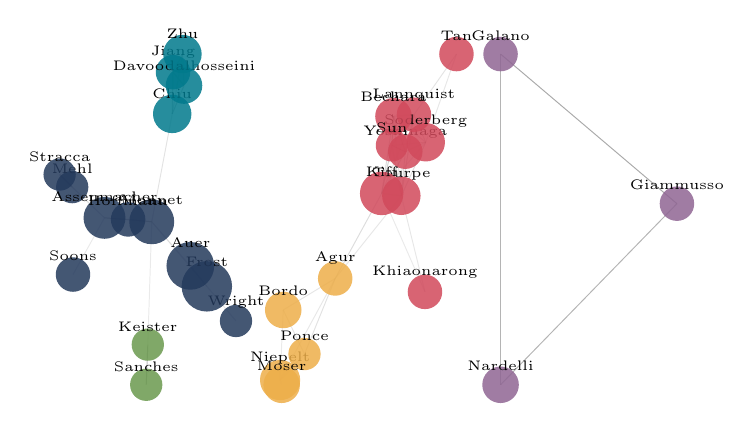
\begin{tikzpicture}
\draw[gray, opacity=0.67, line width=0.35pt] (5.60,4.20) -- (7.84,2.30);
\draw[gray, opacity=0.59, line width=0.35pt] (5.60,4.20) -- (5.60,0.00);
\draw[gray, opacity=0.59, line width=0.35pt] (5.60,0.00) -- (7.84,2.30);
\draw[gray, opacity=0.56, line width=0.35pt] (4.39,2.96) -- (4.22,3.04);
\draw[gray, opacity=0.52, line width=0.35pt] (0.16,2.51) -- (0.00,2.67);
\draw[gray, opacity=0.52, line width=0.35pt] (1.10,0.00) -- (1.12,0.51);
\draw[gray, opacity=0.51, line width=0.35pt] (4.39,2.96) -- (4.24,3.41);
\draw[gray, opacity=0.50, line width=0.35pt] (4.24,3.41) -- (4.22,3.04);
\draw[gray, opacity=0.43, line width=0.35pt] (1.44,3.97) -- (1.58,3.80);
\draw[gray, opacity=0.41, line width=0.35pt] (1.43,3.44) -- (1.58,3.80);
\draw[gray, opacity=0.40, line width=0.35pt] (1.44,3.97) -- (1.43,3.44);
\draw[gray, opacity=0.40, line width=0.35pt] (1.44,3.97) -- (1.56,4.20);
\draw[gray, opacity=0.36, line width=0.35pt] (4.09,2.43) -- (4.22,3.04);
\draw[gray, opacity=0.36, line width=0.35pt] (4.50,3.43) -- (4.24,3.41);
\draw[gray, opacity=0.34, line width=0.35pt] (4.50,3.43) -- (4.22,3.04);
\draw[gray, opacity=0.33, line width=0.35pt] (4.50,3.43) -- (4.34,2.40);
\draw[gray, opacity=0.32, line width=0.35pt] (4.39,2.96) -- (4.09,2.43);
\draw[gray, opacity=0.30, line width=0.35pt] (4.39,2.96) -- (4.50,3.43);
\draw[gray, opacity=0.30, line width=0.35pt] (1.17,2.07) -- (0.87,2.10);
\draw[gray, opacity=0.30, line width=0.35pt] (1.58,3.80) -- (1.56,4.20);
\draw[gray, opacity=0.29, line width=0.35pt] (4.09,2.43) -- (4.24,3.41);
\draw[gray, opacity=0.29, line width=0.35pt] (4.65,3.08) -- (4.22,3.04);
\draw[gray, opacity=0.29, line width=0.35pt] (4.34,2.40) -- (4.22,3.04);
\draw[gray, opacity=0.29, line width=0.35pt] (0.57,2.12) -- (0.87,2.10);
\draw[gray, opacity=0.27, line width=0.35pt] (4.65,3.08) -- (4.34,2.40);
\draw[gray, opacity=0.27, line width=0.35pt] (1.43,3.44) -- (1.56,4.20);
\draw[gray, opacity=0.27, line width=0.35pt] (4.34,2.40) -- (4.09,2.43);
\draw[gray, opacity=0.27, line width=0.35pt] (3.50,1.35) -- (4.09,2.43);
\draw[gray, opacity=0.26, line width=0.35pt] (4.39,2.96) -- (4.65,3.08);
\draw[gray, opacity=0.26, line width=0.35pt] (4.39,2.96) -- (4.34,2.40);
\draw[gray, opacity=0.26, line width=0.35pt] (4.50,3.43) -- (4.65,3.08);
\draw[gray, opacity=0.25, line width=0.35pt] (1.87,1.25) -- (1.66,1.51);
\draw[gray, opacity=0.25, line width=0.35pt] (0.16,2.51) -- (0.57,2.12);
\draw[gray, opacity=0.24, line width=0.35pt] (4.65,3.08) -- (4.24,3.41);
\draw[gray, opacity=0.24, line width=0.35pt] (4.34,2.40) -- (4.24,3.41);
\draw[gray, opacity=0.23, line width=0.35pt] (3.50,1.35) -- (3.11,0.39);
\draw[gray, opacity=0.22, line width=0.35pt] (1.17,2.07) -- (1.43,3.44);
\draw[gray, opacity=0.22, line width=0.35pt] (4.50,3.43) -- (4.09,2.43);
\draw[gray, opacity=0.21, line width=0.35pt] (3.11,0.39) -- (2.84,0.95);
\draw[gray, opacity=0.21, line width=0.35pt] (4.50,3.43) -- (5.04,4.20);
\draw[gray, opacity=0.20, line width=0.35pt] (2.24,0.81) -- (1.87,1.25);
\draw[gray, opacity=0.20, line width=0.35pt] (1.17,2.07) -- (0.57,2.12);
\draw[gray, opacity=0.20, line width=0.35pt] (3.50,1.35) -- (2.84,0.95);
\draw[gray, opacity=0.20, line width=0.35pt] (4.65,3.08) -- (4.09,2.43);
\draw[gray, opacity=0.19, line width=0.35pt] (2.80,0.06) -- (3.11,0.39);
\draw[gray, opacity=0.19, line width=0.35pt] (5.04,4.20) -- (4.65,3.08);
\draw[gray, opacity=0.19, line width=0.35pt] (4.34,2.40) -- (3.50,1.35);
\draw[gray, opacity=0.19, line width=0.35pt] (4.34,2.40) -- (4.64,1.18);
\draw[gray, opacity=0.18, line width=0.35pt] (2.80,0.06) -- (3.50,1.35);
\draw[gray, opacity=0.17, line width=0.35pt] (1.17,2.07) -- (1.12,0.51);
\draw[gray, opacity=0.17, line width=0.35pt] (0.57,2.12) -- (0.17,1.40);
\draw[gray, opacity=0.17, line width=0.35pt] (2.80,0.06) -- (2.84,0.95);
\draw[gray, opacity=0.17, line width=0.35pt] (2.80,0.06) -- (2.82,0.00);
\draw[gray, opacity=0.17, line width=0.35pt] (4.09,2.43) -- (4.64,1.18);
\draw[gray, opacity=0.16, line width=0.35pt] (1.17,2.07) -- (1.66,1.51);
\draw[gray, opacity=0.15, line width=0.35pt] (1.17,2.07) -- (1.87,1.25);
\fill[c2, opacity=0.85] (4.39,2.96) circle (2.19mm);
\node[font=\fontsize{4.6}{5}\selectfont, above=1.53mm, inner sep=0.5pt] at (4.39,2.96) {Yoshinaga};
\fill[c1, opacity=0.85] (2.24,0.81) circle (2.05mm);
\node[font=\fontsize{4.6}{5}\selectfont, above=1.44mm, inner sep=0.5pt] at (2.24,0.81) {Wright};
\fill[c1, opacity=0.85] (0.16,2.51) circle (2.05mm);
\node[font=\fontsize{4.6}{5}\selectfont, above=1.44mm, inner sep=0.5pt] at (0.16,2.51) {Mehl};
\fill[c2, opacity=0.85] (4.50,3.43) circle (2.19mm);
\node[font=\fontsize{4.6}{5}\selectfont, above=1.53mm, inner sep=0.5pt] at (4.50,3.43) {Lannquist};
\fill[c2, opacity=0.85] (5.04,4.20) circle (2.19mm);
\node[font=\fontsize{4.6}{5}\selectfont, above=1.53mm, inner sep=0.5pt] at (5.04,4.20) {Tan};
\fill[c1, opacity=0.85] (1.17,2.07) circle (2.85mm);
\node[font=\fontsize{4.6}{5}\selectfont, above=2.00mm, inner sep=0.5pt] at (1.17,2.07) {Monnet};
\fill[c6, opacity=0.85] (1.10,0.00) circle (2.05mm);
\node[font=\fontsize{4.6}{5}\selectfont, above=1.44mm, inner sep=0.5pt] at (1.10,0.00) {Sanches};
\fill[c3, opacity=0.85] (2.80,0.06) circle (2.55mm);
\node[font=\fontsize{4.6}{5}\selectfont, above=1.79mm, inner sep=0.5pt] at (2.80,0.06) {Niepelt};
\fill[c2, opacity=0.85] (4.65,3.08) circle (2.44mm);
\node[font=\fontsize{4.6}{5}\selectfont, above=1.71mm, inner sep=0.5pt] at (4.65,3.08) {Soderberg};
\fill[c5, opacity=0.85] (5.60,4.20) circle (2.19mm);
\node[font=\fontsize{4.6}{5}\selectfont, above=1.53mm, inner sep=0.5pt] at (5.60,4.20) {Galano};
\fill[c2, opacity=0.85] (4.34,2.40) circle (2.44mm);
\node[font=\fontsize{4.6}{5}\selectfont, above=1.71mm, inner sep=0.5pt] at (4.34,2.40) {Tourpe};
\fill[c3, opacity=0.85] (3.50,1.35) circle (2.19mm);
\node[font=\fontsize{4.6}{5}\selectfont, above=1.53mm, inner sep=0.5pt] at (3.50,1.35) {Agur};
\fill[c4, opacity=0.85] (1.44,3.97) circle (2.19mm);
\node[font=\fontsize{4.6}{5}\selectfont, above=1.53mm, inner sep=0.5pt] at (1.44,3.97) {Jiang};
\fill[c2, opacity=0.85] (4.09,2.43) circle (2.76mm);
\node[font=\fontsize{4.6}{5}\selectfont, above=1.93mm, inner sep=0.5pt] at (4.09,2.43) {Kiff};
\fill[c1, opacity=0.85] (1.87,1.25) circle (3.20mm);
\node[font=\fontsize{4.6}{5}\selectfont, above=2.24mm, inner sep=0.5pt] at (1.87,1.25) {Frost};
\fill[c4, opacity=0.85] (1.43,3.44) circle (2.44mm);
\node[font=\fontsize{4.6}{5}\selectfont, above=1.71mm, inner sep=0.5pt] at (1.43,3.44) {Chiu};
\fill[c3, opacity=0.85] (3.11,0.39) circle (2.05mm);
\node[font=\fontsize{4.6}{5}\selectfont, above=1.44mm, inner sep=0.5pt] at (3.11,0.39) {Ponce};
\fill[c1, opacity=0.85] (0.57,2.12) circle (2.66mm);
\node[font=\fontsize{4.6}{5}\selectfont, above=1.86mm, inner sep=0.5pt] at (0.57,2.12) {Assenmacher};
\fill[c1, opacity=0.85] (0.00,2.67) circle (2.05mm);
\node[font=\fontsize{4.6}{5}\selectfont, above=1.44mm, inner sep=0.5pt] at (0.00,2.67) {Stracca};
\fill[c2, opacity=0.85] (4.24,3.41) circle (2.32mm);
\node[font=\fontsize{4.6}{5}\selectfont, above=1.62mm, inner sep=0.5pt] at (4.24,3.41) {Bechara};
\fill[c5, opacity=0.85] (5.60,0.00) circle (2.32mm);
\node[font=\fontsize{4.6}{5}\selectfont, above=1.62mm, inner sep=0.5pt] at (5.60,0.00) {Nardelli};
\fill[c3, opacity=0.85] (2.84,0.95) circle (2.32mm);
\node[font=\fontsize{4.6}{5}\selectfont, above=1.62mm, inner sep=0.5pt] at (2.84,0.95) {Bordo};
\fill[c1, opacity=0.85] (0.17,1.40) circle (2.19mm);
\node[font=\fontsize{4.6}{5}\selectfont, above=1.53mm, inner sep=0.5pt] at (0.17,1.40) {Soons};
\fill[c1, opacity=0.85] (0.87,2.10) circle (2.19mm);
\node[font=\fontsize{4.6}{5}\selectfont, above=1.53mm, inner sep=0.5pt] at (0.87,2.10) {Hoffmann};
\fill[c1, opacity=0.85] (1.66,1.51) circle (3.03mm);
\node[font=\fontsize{4.6}{5}\selectfont, above=2.12mm, inner sep=0.5pt] at (1.66,1.51) {Auer};
\fill[c5, opacity=0.85] (7.84,2.30) circle (2.19mm);
\node[font=\fontsize{4.6}{5}\selectfont, above=1.53mm, inner sep=0.5pt] at (7.84,2.30) {Giammusso};
\fill[c4, opacity=0.85] (1.58,3.80) circle (2.32mm);
\node[font=\fontsize{4.6}{5}\selectfont, above=1.62mm, inner sep=0.5pt] at (1.58,3.80) {Davoodalhosseini};
\fill[c2, opacity=0.85] (4.64,1.18) circle (2.19mm);
\node[font=\fontsize{4.6}{5}\selectfont, above=1.53mm, inner sep=0.5pt] at (4.64,1.18) {Khiaonarong};
\fill[c2, opacity=0.85] (4.22,3.04) circle (2.05mm);
\node[font=\fontsize{4.6}{5}\selectfont, above=1.44mm, inner sep=0.5pt] at (4.22,3.04) {Sun};
\fill[c3, opacity=0.85] (2.82,0.00) circle (2.32mm);
\node[font=\fontsize{4.6}{5}\selectfont, above=1.62mm, inner sep=0.5pt] at (2.82,0.00) {Moser};
\fill[c6, opacity=0.85] (1.12,0.51) circle (2.05mm);
\node[font=\fontsize{4.6}{5}\selectfont, above=1.44mm, inner sep=0.5pt] at (1.12,0.51) {Keister};
\fill[c4, opacity=0.85] (1.56,4.20) circle (2.44mm);
\node[font=\fontsize{4.6}{5}\selectfont, above=1.71mm, inner sep=0.5pt] at (1.56,4.20) {Zhu};
\end{tikzpicture}
\end{column}
\begin{column}{0.36\textwidth}\scriptsize
\textbf{Most productive authors}\\[2pt]
\begin{tabular}{@{}lr@{}}Ulrich Bindseil & 20 \\
Peterson K Ozili & 20 \\
Jon Frost & 16 \\
Annelieke Mooij & 16 \\
Raphael Auer & 14 \\
Cyril Monnet & 12 \\
John Kiff & 11 \\
Katrin Assenmacher & 10 \\\end{tabular}\\[6pt]
5,716 authors; 48\% of papers co-authored (mean team 1.9); 15\% international. Top countries: RU 473, US 248, DE 167, CN 166, GB 153.\\[4pt]
Papers with a central bank, BIS, IMF or World Bank author: \alert{10\%} (23\% in 2014--2019, 7\% in 2023--2026), but \alert{48\% of citations}.
\end{column}
\end{columns}
\method{m:net}
\note{\textbf{Co-authorship (0:45).}}
\end{frame}

\begin{frame}{Who says what: research economists vs central bankers}
\slabel{r:logodds}
\footnotesize
Words most over-used by each group compared with the other ($z$-scores):\\[4pt]
\begin{tabular}{@{}p{0.42\textwidth}p{0.42\textwidth}@{}}\toprule
\textbf{Research economists} \scriptsize(259,105 words) & \textbf{Central bankers} \scriptsize(232,446 words)\\\midrule
legal \hfill 23 & payments \hfill 28 \\
analysis \hfill 21 & euro \hfill 22 \\
development \hfill 21 & european \hfill 18 \\
research \hfill 20 & europe \hfill 18 \\
monetary \hfill 20 & area \hfill 18 \\
impact \hfill 19 & services \hfill 15 \\
model \hfill 18 & innovation \hfill 14 \\
implementation \hfill 17 & conference \hfill 14 \\
\bottomrule\end{tabular}\\[4pt]
\scriptsize English texts; research: title + abstract; central bankers: speeches; topic words (\emph{CBDC, digital, currency\dots}) removed.\\[3pt]
\small \alert{Reading}: research economists: \emph{legal, analysis, development}; central bankers: \emph{payments, euro, european}.
\method{m:logodds}
\note{\textbf{Framing (0:40).}}
\end{frame}

% =====================================================================
\section{What is written}

\begin{frame}{Thematic map: which themes drive the field?}
\slabel{r:thematic}
\begin{columns}[c]
\begin{column}{0.47\textwidth}
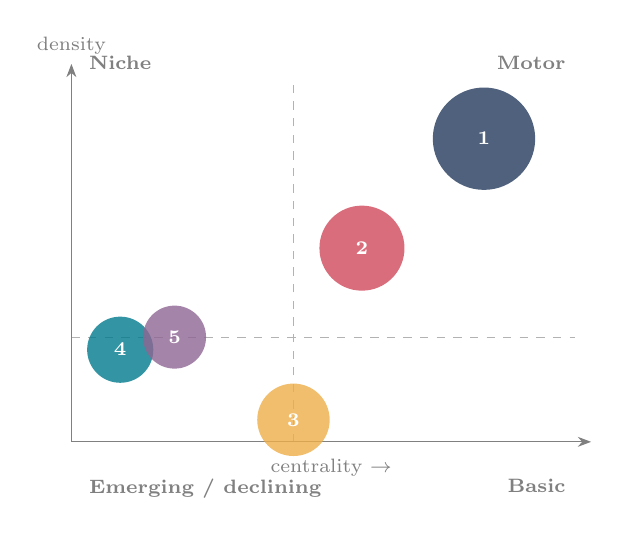
\begin{tikzpicture}[font=\scriptsize]
\draw[gray!60, dashed] (2.82,0) -- (2.82,4.6);
\draw[gray!60, dashed] (0,1.33) -- (6.4,1.33);
\draw[-{Stealth}, gray] (0,0) -- (6.6000000000000005,0) node[below, text=gray, pos=0.5, yshift=-1mm] {centrality $\to$};
\draw[-{Stealth}, gray] (0,0) -- (0,4.8) node[above, text=gray] {density};
\node[gray, anchor=south east, font=\scriptsize\bfseries] at (6.4,4.6) {Motor};
\node[gray, anchor=south west, font=\scriptsize\bfseries] at (0.1,4.6) {Niche};
\node[gray, anchor=north west, font=\scriptsize\bfseries] at (0.1,-0.35) {Emerging / declining};
\node[gray, anchor=north east, font=\scriptsize\bfseries] at (6.4,-0.35) {Basic};
\fill[c1, opacity=0.8] (5.24,3.85) circle (6.5mm);
\node[font=\scriptsize, text=white] at (5.24,3.85) {\textbf{1}};
\fill[c2, opacity=0.8] (3.69,2.46) circle (5.4mm);
\node[font=\scriptsize, text=white] at (3.69,2.46) {\textbf{2}};
\fill[c3, opacity=0.8] (2.82,0.28) circle (4.6mm);
\node[font=\scriptsize, text=white] at (2.82,0.28) {\textbf{3}};
\fill[c4, opacity=0.8] (0.62,1.17) circle (4.2mm);
\node[font=\scriptsize, text=white] at (0.62,1.17) {\textbf{4}};
\fill[c5, opacity=0.8] (1.31,1.33) circle (4.0mm);
\node[font=\scriptsize, text=white] at (1.31,1.33) {\textbf{5}};
\end{tikzpicture}
\end{column}
\begin{column}{0.51\textwidth}\scriptsize
Keyword clusters placed by \alert{centrality} (links to other themes) and \alert{density} (internal cohesion).\\[3pt]
\begin{tabular}{@{}lp{0.62\linewidth}l@{}}\toprule
 & \textbf{Theme} (top keywords) & \textbf{Quadrant}\\\midrule
\textcolor{c1}{\textbf{1}} & digital transformation in financial services, monetary policy, moneta\dots{} & motor \\
\textcolor{c2}{\textbf{2}} & blockchain technology applications and security, digital transformati\dots{} & motor \\
\textcolor{c3}{\textbf{3}} & fintech, crowdfunding, digital finance, blockchain, fintech & basic \\
\textcolor{c4}{\textbf{4}} & global financial crisis and policies, international payments, stablec\dots{} & emerging or declining \\
\textcolor{c5}{\textbf{5}} & financial inclusion, digital payments, india & niche \\
\bottomrule\end{tabular}\\[3pt]
\small Motor themes: digital transformation in financial services; blockchain technology applications and security.
\end{column}
\end{columns}
\method{m:callon}
\note{\textbf{Thematic map (0:45).}}
\end{frame}

\begin{frame}{How the themes evolve}
\slabel{r:evo}
\scriptsize
\begin{tabular}{@{}p{0.42\textwidth}rrrr@{}}\toprule
\textbf{Keyword} (\% of the period's papers) & \textbf{2014--2019} & \textbf{2020--2022} & \textbf{2023--2026} & \textbf{Change}\\
\textit{papers in period} & \textit{136} & \textit{755} & \textit{2,919} &\\\midrule
financial inclusion & \cellcolor{c1!5}5.9 & \cellcolor{c1!8}8.2 & \cellcolor{c1!15}15.8 & \textcolor{c4}{$+7.6$} \\
digital euro & \cellcolor{c1!2}2.9 & \cellcolor{c1!7}7.8 & \cellcolor{c1!11}11.4 & \textcolor{c4}{$+3.6$} \\
global financial crisis and policies & \cellcolor{c1!2}2.2 & \cellcolor{c1!8}8.7 & \cellcolor{c1!11}11.8 & \textcolor{c4}{$+3.0$} \\
financial stability & \cellcolor{c1!24}24.3 & \cellcolor{c1!12}12.6 & \cellcolor{c1!15}15.6 & \textcolor{c4}{$+3.0$} \\
fintech, crowdfunding, digital finance & \cellcolor{c1!48}48.5 & \cellcolor{c1!48}48.7 & \cellcolor{c1!49}49.8 & \textcolor{c4}{$+1.0$} \\
digital ruble & \cellcolor{c1!0}0.0 & \cellcolor{c1!13}13.9 & \cellcolor{c1!14}14.8 & \textcolor{c4}{$+0.9$} \\
european monetary and fiscal policies & \cellcolor{c1!16}16.9 & \cellcolor{c1!10}10.3 & \cellcolor{c1!10}10.3 & \textcolor{c2}{$-0.1$} \\
digital transformation in financial ser\dots{} & \cellcolor{c1!60}72.1 & \cellcolor{c1!60}74.7 & \cellcolor{c1!60}74.2 & \textcolor{c2}{$-0.5$} \\
digital transformation in law & \cellcolor{c1!10}10.3 & \cellcolor{c1!17}17.9 & \cellcolor{c1!17}17.3 & \textcolor{c2}{$-0.6$} \\
banking stability, regulation, efficien\dots{} & \cellcolor{c1!22}22.1 & \cellcolor{c1!16}16.4 & \cellcolor{c1!15}15.5 & \textcolor{c2}{$-0.9$} \\
monetary policy and economic impact & \cellcolor{c1!51}51.5 & \cellcolor{c1!23}23.0 & \cellcolor{c1!20}20.7 & \textcolor{c2}{$-2.4$} \\
digital payments & \cellcolor{c1!8}8.8 & \cellcolor{c1!12}12.6 & \cellcolor{c1!10}10.2 & \textcolor{c2}{$-2.4$} \\
\bottomrule\end{tabular}\\[4pt]
Sorted by change between the last two periods. Darker = more frequent.\\[3pt]
\textbf{New in each period} (c-TF-IDF, periods as classes): \textbf{2014--2019}: \emph{e-krona, riksbank, issue, legal, innovation, services}; \textbf{2020--2022}: \emph{euro, ruble, china, legal, interest, national}; \textbf{2023--2026}: \emph{euro, legal, ruble, regulatory, india, data}.\\[2pt]
\small Rising fastest: \alert{financial inclusion}; falling most: \alert{digital payments}.
\method{m:ctfidf}
\note{\textbf{Evolution (0:35).}}
\end{frame}

\begin{frame}{Topics found by meaning (SBERT + BERTopic)}
\slabel{r:topics}
\scriptsize
\setlength{\tabcolsep}{4pt}
\begin{tabular}{@{}rp{0.4\textwidth}rrrrrr@{}}\toprule
 & \textbf{Topic} (top c-TF-IDF terms) & \textbf{Texts} & \multicolumn{3}{c}{\textbf{\% of the period's texts}} & \multicolumn{2}{c}{\textbf{Adjusted, points}}\\
 & & & \textbf{2014--2019} & \textbf{2020--2022} & \textbf{2023--2026} & \textbf{change} & \textbf{CB}\\\midrule
1 & cryptocurrencies, implementation, private, tr\dots{} & 470 & \cellcolor{c1!55}18.5 & \cellcolor{c1!40}13.5 & \cellcolor{c1!25}8.5 & \textbf{-13.2} & \textbf{-8.6} \\
2 & design, retail, legal, private & 439 & \cellcolor{c1!31}10.4 & \cellcolor{c1!33}11.2 & \cellcolor{c1!25}8.6 & {-4.0} & \textbf{-9.4} \\
3 & uncertainty, rates, design, rate & 349 & \cellcolor{c1!42}14.2 & \cellcolor{c1!26}8.7 & \cellcolor{c1!20}6.7 & \textbf{-9.6} & \textbf{-5.9} \\
4 & dollar, trade, debt, reserve & 326 & \cellcolor{c1!17}5.7 & \cellcolor{c1!17}5.8 & \cellcolor{c1!22}7.5 & {+0.8} & \textbf{-5.0} \\
5 & deposits, interest, deposit, rate & 319 & \cellcolor{c1!8}2.8 & \cellcolor{c1!15}5.0 & \cellcolor{c1!21}7.3 & {+3.6} & \textbf{-7.7} \\
6 & governor, innovation, fintech, kong & 306 & \cellcolor{c1!52}17.5 & \cellcolor{c1!33}11.2 & \cellcolor{c1!14}4.7 & {-1.2} & \textbf{+35.7} \\
7 & russian, russia, ruble, federation & 238 & \cellcolor{c1!0}0.0 & \cellcolor{c1!15}5.1 & \cellcolor{c1!14}4.9 & \textbf{+4.7} & \textbf{-5.2} \\
8 & china, rmb, e-cny, yuan & 213 & \cellcolor{c1!4}1.4 & \cellcolor{c1!16}5.3 & \cellcolor{c1!13}4.6 & {+2.7} & \textbf{-5.2} \\
9 & cashless, evolution, riksbank, forms & 204 & \cellcolor{c1!19}6.6 & \cellcolor{c1!14}4.9 & \cellcolor{c1!12}4.1 & \textbf{-3.8} & \textbf{-1.8} \\
10 & fintech, technologies, services, innovation & 199 & \cellcolor{c1!21}7.1 & \cellcolor{c1!8}2.9 & \cellcolor{c1!13}4.4 & \textbf{-3.0} & {-0.5} \\
11 & euro, european, ecb, area & 186 & \cellcolor{c1!1}0.5 & \cellcolor{c1!10}3.6 & \cellcolor{c1!12}4.2 & \textbf{+3.7} & \textbf{+5.6} \\
12 & cryptocurrencies, crypto, bitcoin, cryptocurr\dots{} & 186 & \cellcolor{c1!27}9.0 & \cellcolor{c1!12}4.0 & \cellcolor{c1!10}3.6 & \textbf{-5.8} & {-1.1} \\
\bottomrule\end{tabular}\\[3pt]
4,710 texts; 24 topics (50\% outliers reassigned). Adjusted: logit on period, actor, English; change = 2023--26 vs 2014--19; CB = central banks vs research; \textbf{bold}: 95\% CI excludes 0.\\[2pt]
\small Topics tied to \alert{one jurisdiction}: 6--34\% of texts in every period, but the mix shifts:  fall; \emph{russian}, \emph{euro}, \emph{india} rise.
\method{m:bertopic}
\note{\textbf{Topics (1:00).} Embeddings group texts by meaning across languages; the literature follows national projects.}
\end{frame}

% =====================================================================
\section{How: tone and stance}

\begin{frame}{Tone: how positive is what economists say about CBDCs?}
\slabel{r:tone}
\begin{columns}[T]
\begin{column}{0.46\textwidth}
\begin{tikzpicture}
\begin{axis}[width=\textwidth, height=0.62\textheight, xtick={2019,2020,2021,2022,2023,2024,2025,2026}, xticklabel style={/pgf/number format/1000 sep=, font=\tiny, rotate=45, anchor=north east, inner sep=1pt},
  yticklabel style={font=\scriptsize, /pgf/number format/fixed}, ylabel={net tone}, ylabel style={font=\scriptsize},
  legend style={at={(0.5,-0.18)}, anchor=north, font=\tiny, draw=none, legend columns=2}, axis lines*=left, ymajorgrids]
\addplot[c1, thick, mark=*, mark size=1.2pt] coordinates {(2019,0.071) (2020,0.117) (2021,0.141) (2022,0.167) (2023,0.144) (2024,0.208) (2025,0.247) (2026,0.205)};
\addlegendentry{Research economists}
\addplot[c2, thick, mark=*, mark size=1.2pt] coordinates {(2019,0.075) (2020,0.174) (2021,0.218) (2022,0.236) (2023,0.183) (2024,0.253) (2025,0.297) (2026,0.244)};
\addlegendentry{Central banks \& institutions}
\end{axis}
\end{tikzpicture}
\end{column}
\begin{column}{0.52\textwidth}\scriptsize
\setlength{\tabcolsep}{3pt}
\begin{tabular}{@{}p{0.3\linewidth}rrrrr@{}}\toprule
 & \textbf{Texts} & \textbf{Sent.} & \textbf{\%+} & \textbf{\%--} & \textbf{Net tone}\\\midrule
Research economists & 2,306 & 7,519 & 21 & 5 & $0.19 \pm 0.01$ \\
Central banks \& institutions & 630 & 7,576 & 18 & 3 & $0.22 \pm 0.01$ \\
\bottomrule\end{tabular}\\[4pt]
FinBERT on the 15,095 English sentences that name a CBDC. Sentence tone $= P(+) - P(-)$, averaged per text, then per group ($\pm$ 95\% CI). 90 sentences from economists' texts read blind (of 136): agreement 68\%, $\kappa = 0.52$; positive and negative confused 3 times.\\[4pt]
\small \alert{Reading}: tone rises steadily in both groups; research economists from 0.07 in 2019 to 0.25 in 2025; central banks stay slightly more positive.
\end{column}
\end{columns}
\method{m:finbert}
\note{\textbf{Tone (1:00).} Only sentences naming a CBDC are scored: tone about CBDCs, not about the economy.}
\end{frame}

\begin{frame}{Do policy events move the tone?}
\slabel{r:tev}
\begin{columns}[T]
\begin{column}{0.6\textwidth}\scriptsize
\setlength{\tabcolsep}{3pt}
\begin{tabular}{@{}llrrrr@{}}\toprule
\textbf{Date} & \textbf{Event} & \textbf{Before} & \textbf{After} & $\Delta$\textbf{tone} & $p$\\\midrule
Jun 2019 & Facebook announces Libra & 23 & 42 & -0.041 & 0.33 \\
Oct 2020 & ECB digital euro report & 46 & 113 & +0.003 & 0.89 \\
Oct 2020 & Bahamas launches Sand Dollar & 57 & 111 & -0.020 & 0.55 \\
Jul 2021 & ECB investigation phase & 110 & 102 & +0.020 & 0.56 \\
Oct 2021 & Nigeria launches eNaira & 115 & 103 & +0.050 & 0.24 \\
Jan 2022 & Fed CBDC discussion paper & 102 & 122 & +0.022 & 0.51 \\
Mar 2022 & US order on digital assets & 108 & 129 & +0.004 & 0.87 \\
Nov 2022 & India e-rupee pilot & 130 & 128 & +0.011 & 0.71 \\
Feb 2023 & UK digital pound consultation & 132 & 148 & -0.008 & 0.77 \\
Jun 2023 & EU digital euro bill & 145 & 211 & -0.043 & 0.30 \\
Oct 2023 & ECB preparation phase & 169 & 217 & -0.025 & 0.48 \\
Jan 2025 & US order banning a US CBDC & 193 & 230 & +0.018 & 0.60 \\
\bottomrule\end{tabular}
\end{column}
\begin{column}{0.38\textwidth}\small
For each event: mean tone of the texts in the 180 days \emph{after} minus the 180 days \emph{before}. Compared with 500 random dates: $p$ = share of random dates with a larger $|\Delta|$ (95th percentile: 0.084).\\[6pt]
\alert{Result}: 0 of 12 events move the tone (smallest $p$ = 0.24).\\[4pt]
Tone \alert{drifts}, it does not \alert{jump}: no single event explains the rise.
\end{column}
\end{columns}
\method{m:tev}
\note{\textbf{Tone and events (0:50).} A negative result, and an informative one: the change is gradual.}
\end{frame}

\begin{frame}{Stance: for or against CBDCs?}
\slabel{r:stance}
\begin{columns}[T]
\begin{column}{0.44\textwidth}\scriptsize
\textbf{Level}, read by hand, \% [95\% CI]\\[2pt]
\setlength{\tabcolsep}{3pt}
\begin{tabular}{@{}p{0.36\linewidth}rrr@{}}\toprule
 & $n$ & \textbf{Favourable} & \textbf{Critical}\\\midrule
Research economists & 50 & 8 \tiny[3--19] & 2 \tiny[0--10] \\
Central banks \& institutions & 50 & 52 \tiny[39--65] & 6 \tiny[2--16] \\
\bottomrule\end{tabular}\\[6pt]
\small By reading: 52\% of central bank texts are favourable; research economists are mostly \alert{neutral} (90\%): they analyse, central banks advocate.
\end{column}
\begin{column}{0.54\textwidth}\scriptsize
\textbf{Change} (local LLM, 575 texts sampled per actor $\times$ period), \% favourable\\[2pt]
\setlength{\tabcolsep}{3pt}
\begin{tabular}{@{}p{0.27\linewidth}rrrr@{}}\toprule
 & \textbf{2014--2019} & \textbf{2020--2022} & \textbf{2023--2026} & \textbf{Change, pts}\\\midrule
Research economists & 26 & 38 & 40 & \textbf{+14} \tiny[+1, +27] \\
Central banks \& institutions & 25 & 54 & 65 & \textbf{+40} \tiny[+26, +53] \\
\bottomrule\end{tabular}\\[4pt]
The LLM ($\kappa = 0.45$ on 100 economists' texts, best of four coders, \usedon{b:stance}) calls 46\% of the hand-coded texts favourable against 30\% by reading: its levels are inflated, so only its \emph{changes} are used. \textbf{Bold}: CI excludes 0.\\[4pt]
\small \alert{Reading}: both groups become more favourable; central banks much more, as their own projects advance.
\end{column}
\end{columns}
\method{m:stance}
\note{\textbf{Stance (1:00).} Tone = how positive the words are; stance = whether the author is for or against.}
\end{frame}

% =====================================================================
\section{Why: stated motivations}

\begin{frame}[fragile]{Coding stated motivations}
\slabel{r:codebook}
\begin{columns}[T]
\begin{column}{0.53\textwidth}
\begin{lstlisting}
MOTIVES = {
  "Financial inclusion":
      r"financial\s+inclusion|unbanked|underbanked"
      r"|access\s+to\s+(?:financial\s+services|finance)",
  "Monetary sovereignty":
      r"monetary\s+sovereignty|global\s+stablecoin"
      r"|\blibra\b|big\s*tech|dollari[sz]ation",
  "Decline of cash":
      r"declin\w*\s+(?:in|of)\s+(?:the\s+)?cash"
      r"|cashless|use\s+of\s+cash",
  ...
}
\end{lstlisting}
\end{column}
\begin{column}{0.44\textwidth}\small
\begin{itemize}
\item Motivations are stated in the \alert{introduction} (else abstract, else opening).
\item 10 motivations; codebook built by reading introductions; several per text allowed.
\item 4,110 texts coded; 76\% state at least one.
\item Validated on the 50 held-out texts by economists (of 74; reading-based coding, AI-assisted): precision 0.70, recall 0.41, $\kappa = 0.46$.
\end{itemize}
\end{column}
\end{columns}
\method{m:codebook}
\note{\textbf{Motivations: method (0:35).}}
\end{frame}

\begin{frame}{Why: what economists say CBDCs are for}
\slabel{r:motives}
\scriptsize
\setlength{\tabcolsep}{4pt}
\begin{tabular}{@{}p{0.29\textwidth}rrrrr@{}}\toprule
 & \multicolumn{3}{c}{\textbf{\% of texts}} & \multicolumn{2}{c}{\textbf{Adjusted effect, points [95\% CI]}}\\
\textbf{Motivation} & \textbf{2014--2019} & \textbf{2020--2022} & \textbf{2023--2026} & \textbf{Change} & \textbf{Central banks}\\
 & & & & \textbf{2023--26 vs 2014--19} & \textbf{vs research}\\\midrule
Financial stability & \cellcolor{c1!46}30.8 & \cellcolor{c1!39}26.3 & \cellcolor{c1!43}29.3 & {-1.6} \tiny[-8, +5] & \textbf{-7.7} \tiny[-11, -4] \\
Monetary policy & \cellcolor{c1!55}36.8 & \cellcolor{c1!41}27.4 & \cellcolor{c1!36}24.4 & \textbf{-15.1} \tiny[-22, -8] & \textbf{-13.6} \tiny[-16, -11] \\
Technology (DLT, programmability) & \cellcolor{c1!33}22.5 & \cellcolor{c1!32}21.6 & \cellcolor{c1!38}25.8 & {+1.6} \tiny[-5, +8] & \textbf{-9.1} \tiny[-12, -6] \\
Cross-border payments & \cellcolor{c1!19}13.2 & \cellcolor{c1!28}19.0 & \cellcolor{c1!33}22.5 & \textbf{+8.7} \tiny[+3, +13] & \textbf{-7.8} \tiny[-11, -5] \\
Payment efficiency & \cellcolor{c1!15}10.4 & \cellcolor{c1!18}12.1 & \cellcolor{c1!26}17.4 & \textbf{+6.6} \tiny[+1, +11] & \textbf{-3.1} \tiny[-6, -0] \\
Monetary sovereignty & \cellcolor{c1!23}15.9 & \cellcolor{c1!25}16.8 & \cellcolor{c1!20}13.6 & {-2.0} \tiny[-8, +3] & {-2.4} \tiny[-5, +0] \\
Financial inclusion & \cellcolor{c1!5}3.8 & \cellcolor{c1!13}8.9 & \cellcolor{c1!25}16.8 & \textbf{+12.3} \tiny[+8, +15] & \textbf{-9.5} \tiny[-12, -7] \\
Geopolitics and sanctions & \cellcolor{c1!4}2.7 & \cellcolor{c1!10}7.2 & \cellcolor{c1!22}15.0 & \textbf{+12.4} \tiny[+9, +15] & {+0.3} \tiny[-2, +3] \\
Privacy and surveillance & \cellcolor{c1!10}7.1 & \cellcolor{c1!15}10.5 & \cellcolor{c1!20}13.6 & \textbf{+6.4} \tiny[+2, +10] & \textbf{-2.8} \tiny[-5, -0] \\
Decline of cash & \cellcolor{c1!22}14.8 & \cellcolor{c1!13}9.0 & \cellcolor{c1!11}7.4 & \textbf{-6.5} \tiny[-12, -2] & {+1.2} \tiny[-1, +4] \\
\bottomrule\end{tabular}\\[3pt]
Logit of each motivation on period, actor and English; average marginal effects, robust SEs. \textbf{Bold}: CI excludes 0.
\begin{itemize}\setlength\itemsep{0pt}
\item \alert{Rising:} geopolitics and sanctions ($+12$\,pts), financial inclusion ($+12$\,pts), cross-border payments ($+9$\,pts). \quad \alert{Falling:} monetary policy ($-15$\,pts), decline of cash ($-7$\,pts).
\item From a \alert{monetary-policy instrument} to a tool for \alert{inclusion, payments and geopolitics}. Recall $\approx 0.41$: shares are \alert{lower bounds}; compare motivations and periods rather than read levels.
\end{itemize}
\method{m:logit}
\note{\textbf{Motivations: results (1:00).}}
\end{frame}

\begin{frame}{Is the codebook the best coder?}
\slabel{r:coders}
\begin{columns}[T]
\begin{column}{0.58\textwidth}\scriptsize
\begin{tabular}{@{}lrrrrr@{}}\toprule
\textbf{Coder} & \textbf{P} & \textbf{R} & $F_1$ & $\kappa$ & $\kappa$\textbf{, all}\\\midrule
\rowcolor{c4!12}Codebook (regex) & 0.70 & 0.41 & 0.52 & 0.46 & 0.50 \\
Codebook OR classifier & 0.42 & 0.60 & 0.50 & 0.39 & 0.42 \\
SBERT, classifier (100 labels) & 0.36 & 0.37 & 0.37 & 0.25 & 0.28 \\
Local LLM, Qwen2.5 7B & 0.30 & 0.61 & 0.40 & 0.25 & 0.28 \\
Local LLM, Qwen2.5 3B & 0.31 & 0.23 & 0.26 & 0.15 & 0.16 \\
SBERT, definitions (zero-shot) & 0.21 & 0.71 & 0.32 & 0.12 & 0.15 \\
NLI zero-shot (mDeBERTa) & 0.22 & 0.39 & 0.28 & 0.11 & 0.14 \\
\bottomrule\end{tabular}\\[3pt]
The 50 held-out texts written by economists $\times$ 10 motivations; last column: $\kappa$ on all 74 held-out texts. Thresholds and classifiers set on 100 development texts.
\end{column}
\begin{column}{0.4\textwidth}\small
\begin{itemize}\setlength\itemsep{2pt}
\item \alert{The codebook wins}: $\kappa = 0.46$; best alternative 0.25.
\item Models confuse ``mentions privacy'' with ``studies CBDCs because of privacy''.
\item Trends hold: same direction of change for 9 of 10 motivations with the high-recall coding, 9 of 10 on main-theme texts only.
\end{itemize}
\end{column}
\end{columns}
\method{m:codebook}
\note{\textbf{Measuring motivations (0:35).}}
\end{frame}

% =====================================================================
\section{When: the environment}

\begin{frame}{Which themes burst, and when}
\slabel{r:burst}
\hspace*{3.3cm}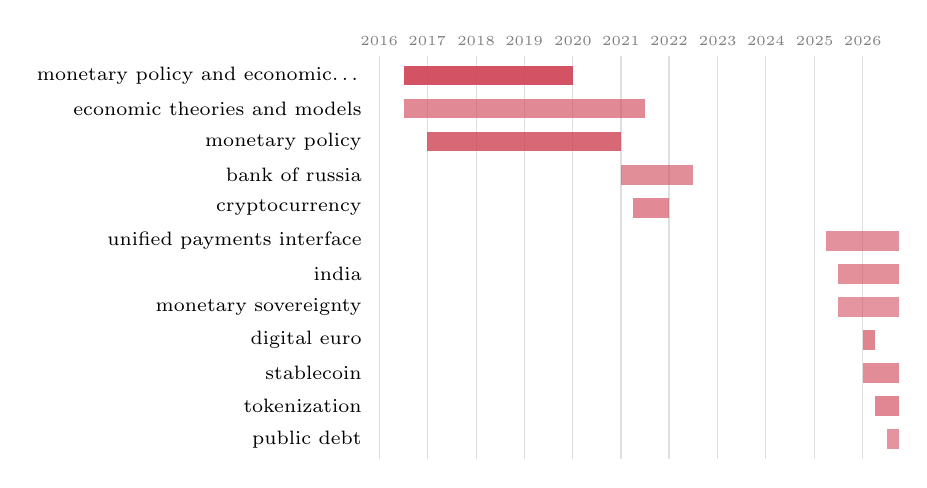
\begin{tikzpicture}[font=\scriptsize, y=-0.42cm]
\draw[gray!25] (0.00,-0.6) -- (0.00,11.60); \node[gray, above, font=\tiny] at (0.00,-0.6) {2016};
\draw[gray!25] (0.61,-0.6) -- (0.61,11.60); \node[gray, above, font=\tiny] at (0.61,-0.6) {2017};
\draw[gray!25] (1.23,-0.6) -- (1.23,11.60); \node[gray, above, font=\tiny] at (1.23,-0.6) {2018};
\draw[gray!25] (1.84,-0.6) -- (1.84,11.60); \node[gray, above, font=\tiny] at (1.84,-0.6) {2019};
\draw[gray!25] (2.46,-0.6) -- (2.46,11.60); \node[gray, above, font=\tiny] at (2.46,-0.6) {2020};
\draw[gray!25] (3.07,-0.6) -- (3.07,11.60); \node[gray, above, font=\tiny] at (3.07,-0.6) {2021};
\draw[gray!25] (3.68,-0.6) -- (3.68,11.60); \node[gray, above, font=\tiny] at (3.68,-0.6) {2022};
\draw[gray!25] (4.30,-0.6) -- (4.30,11.60); \node[gray, above, font=\tiny] at (4.30,-0.6) {2023};
\draw[gray!25] (4.91,-0.6) -- (4.91,11.60); \node[gray, above, font=\tiny] at (4.91,-0.6) {2024};
\draw[gray!25] (5.53,-0.6) -- (5.53,11.60); \node[gray, above, font=\tiny] at (5.53,-0.6) {2025};
\draw[gray!25] (6.14,-0.6) -- (6.14,11.60); \node[gray, above, font=\tiny] at (6.14,-0.6) {2026};
\node[anchor=east] at (-0.1,0) {monetary policy and economic\dots{}};
\fill[c2, opacity=0.95] (0.31,-0.3) rectangle (2.46,0.3);
\node[anchor=east] at (-0.1,1) {economic theories and models};
\fill[c2, opacity=0.65] (0.31,0.7) rectangle (3.38,1.3);
\node[anchor=east] at (-0.1,2) {monetary policy};
\fill[c2, opacity=0.83] (0.61,1.7) rectangle (3.07,2.3);
\node[anchor=east] at (-0.1,3) {bank of russia};
\fill[c2, opacity=0.62] (3.07,2.7) rectangle (3.99,3.3);
\node[anchor=east] at (-0.1,4) {cryptocurrency};
\fill[c2, opacity=0.65] (3.22,3.7) rectangle (3.68,4.3);
\node[anchor=east] at (-0.1,5) {unified payments interface};
\fill[c2, opacity=0.60] (5.68,4.7) rectangle (6.60,5.3);
\node[anchor=east] at (-0.1,6) {india};
\fill[c2, opacity=0.61] (5.83,5.7) rectangle (6.60,6.3);
\node[anchor=east] at (-0.1,7) {monetary sovereignty};
\fill[c2, opacity=0.58] (5.83,6.7) rectangle (6.60,7.3);
\node[anchor=east] at (-0.1,8) {digital euro};
\fill[c2, opacity=0.68] (6.14,7.7) rectangle (6.29,8.3);
\node[anchor=east] at (-0.1,9) {stablecoin};
\fill[c2, opacity=0.63] (6.14,8.7) rectangle (6.60,9.3);
\node[anchor=east] at (-0.1,10) {tokenization};
\fill[c2, opacity=0.66] (6.29,9.7) rectangle (6.60,10.3);
\node[anchor=east] at (-0.1,11) {public debt};
\fill[c2, opacity=0.59] (6.45,10.7) rectangle (6.60,11.3);
\end{tikzpicture}\\[2pt]
\small \alert{Reading}: early bursts on monetary policy and economic impact, economic theories and models, monetary policy; the latest on unified payments interface, india, monetary sovereignty, digital euro.
\method{m:burst}
\note{\textbf{Bursts (0:40).} The data say when a theme suddenly takes off.}
\end{frame}

\begin{frame}{Attention around policy events}
\slabel{r:event}
\begin{columns}[c]
\begin{column}{0.48\textwidth}
\begin{tikzpicture}
\begin{axis}[width=\textwidth, height=0.62\textheight, ymin=0, ymax=\ymaxev, xmin=2019, xmax=2026.85,
  xticklabel style={/pgf/number format/1000 sep=, font=\scriptsize}, xtick={2019,...,2026},
  yticklabel style={font=\scriptsize}, ylabel={texts per week}, ylabel style={font=\scriptsize},
  axis lines*=left, clip=false]
\addplot[c1, thin, const plot] coordinates {(2018.997,1) (2019.016,1) (2019.093,2) (2019.112,2) (2019.131,1) (2019.151,3) (2019.170,2) (2019.208,2) (2019.227,2) (2019.246,2) (2019.266,1) (2019.323,5)
  (2019.342,1) (2019.381,2) (2019.400,2) (2019.419,1) (2019.438,1) (2019.496,2) (2019.515,1) (2019.534,2) (2019.553,2) (2019.572,1) (2019.591,1) (2019.611,1)
  (2019.630,2) (2019.649,3) (2019.668,3) (2019.687,1) (2019.706,2) (2019.726,1) (2019.745,4) (2019.764,1) (2019.783,4) (2019.802,3) (2019.821,2) (2019.841,2)
  (2019.860,1) (2019.879,2) (2019.898,3) (2019.917,5) (2019.936,1) (2019.956,2) (2019.994,1) (2020.014,2) (2020.033,1) (2020.052,2) (2020.071,2) (2020.090,1)
  (2020.110,2) (2020.129,2) (2020.148,6) (2020.167,1) (2020.186,4) (2020.244,3) (2020.282,3) (2020.301,1) (2020.320,4) (2020.339,2) (2020.359,1) (2020.378,1)
  (2020.397,1) (2020.416,2) (2020.435,4) (2020.454,2) (2020.474,2) (2020.493,5) (2020.512,2) (2020.550,2) (2020.569,2) (2020.589,1) (2020.608,3) (2020.627,2)
  (2020.646,1) (2020.665,4) (2020.684,4) (2020.704,2) (2020.723,2) (2020.742,7) (2020.761,6) (2020.780,6) (2020.799,6) (2020.819,9) (2020.838,7) (2020.857,1)
  (2020.876,3) (2020.895,5) (2020.914,16) (2020.934,14) (2020.953,2) (2020.972,3) (2020.991,9) (2021.008,1) (2021.047,5) (2021.066,2) (2021.085,6) (2021.104,6)
  (2021.123,1) (2021.142,6) (2021.162,8) (2021.181,1) (2021.200,6) (2021.219,6) (2021.238,8) (2021.257,5) (2021.277,3) (2021.296,5) (2021.315,7) (2021.334,4)
  (2021.353,7) (2021.372,5) (2021.392,10) (2021.411,6) (2021.430,7) (2021.449,6) (2021.468,4) (2021.487,15) (2021.507,2) (2021.526,5) (2021.545,4) (2021.564,5)
  (2021.583,6) (2021.602,3) (2021.621,1) (2021.641,4) (2021.660,8) (2021.679,2) (2021.698,8) (2021.717,5) (2021.736,12) (2021.756,4) (2021.775,3) (2021.794,5)
  (2021.813,2) (2021.832,5) (2021.851,6) (2021.871,5) (2021.890,2) (2021.909,8) (2021.928,6) (2021.947,3) (2021.966,2) (2021.986,9) (2022.005,2) (2022.025,3)
  (2022.044,5) (2022.063,3) (2022.082,7) (2022.101,4) (2022.120,6) (2022.140,3) (2022.159,13) (2022.178,1) (2022.197,3) (2022.216,6) (2022.235,9) (2022.255,2)
  (2022.274,3) (2022.293,6) (2022.312,9) (2022.331,3) (2022.350,3) (2022.370,6) (2022.389,6) (2022.408,14) (2022.427,4) (2022.446,7) (2022.465,5) (2022.485,17)
  (2022.504,3) (2022.523,6) (2022.542,2) (2022.561,2) (2022.580,8) (2022.600,3) (2022.619,10) (2022.638,10) (2022.657,15) (2022.676,6) (2022.695,1) (2022.715,1)
  (2022.734,17) (2022.753,3) (2022.772,6) (2022.791,3) (2022.810,2) (2022.830,8) (2022.849,6) (2022.868,7) (2022.887,3) (2022.906,14) (2022.925,4) (2022.945,3)
  (2022.964,6) (2022.983,15) (2023.003,4) (2023.022,3) (2023.041,5) (2023.060,4) (2023.079,10) (2023.099,4) (2023.118,3) (2023.137,6) (2023.156,20) (2023.175,8)
  (2023.214,3) (2023.233,16) (2023.252,5) (2023.271,7) (2023.290,5) (2023.309,12) (2023.329,10) (2023.348,5) (2023.367,12) (2023.386,7) (2023.405,10) (2023.424,7)
  (2023.444,8) (2023.463,11) (2023.482,22) (2023.501,7) (2023.520,6) (2023.539,7) (2023.559,4) (2023.578,9) (2023.597,2) (2023.616,7) (2023.635,7) (2023.654,25)
  (2023.674,10) (2023.693,8) (2023.712,5) (2023.731,17) (2023.750,4) (2023.769,7) (2023.789,40) (2023.808,19) (2023.827,12) (2023.846,6) (2023.865,6) (2023.884,6)
  (2023.903,24) (2023.923,9) (2023.942,5) (2023.961,13) (2023.980,19) (2024.000,8) (2024.019,4) (2024.038,8) (2024.057,8) (2024.077,11) (2024.096,8) (2024.115,25)
  (2024.134,4) (2024.153,11) (2024.172,13) (2024.192,4) (2024.211,10) (2024.230,8) (2024.249,11) (2024.268,9) (2024.287,8) (2024.307,11) (2024.326,16) (2024.345,5)
  (2024.364,5) (2024.383,8) (2024.402,22) (2024.422,10) (2024.441,6) (2024.460,11) (2024.479,19) (2024.498,12) (2024.517,8) (2024.537,6) (2024.556,5) (2024.575,8)
  (2024.594,4) (2024.613,7) (2024.632,4) (2024.652,15) (2024.671,11) (2024.690,8) (2024.709,9) (2024.728,10) (2024.747,16) (2024.767,8) (2024.786,14) (2024.805,11)
  (2024.824,15) (2024.843,7) (2024.862,9) (2024.882,6) (2024.901,20) (2024.920,13) (2024.939,14) (2024.958,2) (2024.977,6) (2024.997,15) (2025.014,4) (2025.033,13)
  (2025.052,10) (2025.071,17) (2025.090,6) (2025.110,7) (2025.129,9) (2025.148,24) (2025.167,6) (2025.186,8) (2025.205,7) (2025.225,4) (2025.244,15) (2025.263,13)
  (2025.282,5) (2025.301,11) (2025.320,15) (2025.339,8) (2025.359,12) (2025.378,6) (2025.397,24) (2025.416,11) (2025.435,9) (2025.454,12) (2025.474,12) (2025.493,22)
  (2025.512,10) (2025.531,10) (2025.550,6) (2025.569,11) (2025.589,7) (2025.608,6) (2025.627,14) (2025.646,12) (2025.665,16) (2025.684,4) (2025.704,6) (2025.723,11)
  (2025.742,27) (2025.761,13) (2025.780,18) (2025.799,10) (2025.819,47) (2025.838,13) (2025.857,15) (2025.876,10) (2025.895,21) (2025.914,26) (2025.934,17) (2025.953,18)
  (2025.972,15) (2025.991,40) (2026.011,11) (2026.030,8) (2026.049,7) (2026.068,20) (2026.088,15) (2026.107,12) (2026.126,24) (2026.145,30) (2026.164,13) (2026.183,21)
  (2026.203,9) (2026.222,14) (2026.241,30) (2026.260,15) (2026.279,19) (2026.298,13) (2026.318,23) (2026.337,18) (2026.356,22) (2026.375,12) (2026.394,27) (2026.413,30)
  (2026.433,16) (2026.452,31) (2026.471,15) (2026.490,31) (2026.509,21) (2026.528,16) (2026.548,12) (2026.567,23) (2026.586,15) (2026.605,15) (2026.624,20) (2026.643,15)
  (2026.663,34) (2026.682,15) (2026.701,8) (2026.720,12) (2026.739,22) (2026.758,20) (2026.816,2)};
\draw[gray, thin] (axis cs:2019.460,0) -- (axis cs:2019.460,\ymaxev) node[above, font=\scriptsize, inner sep=1pt] {1};
\draw[c2, thin] (axis cs:2020.753,0) -- (axis cs:2020.753,0.9*\ymaxev) node[above, font=\scriptsize, inner sep=1pt] {2};
\draw[c2, thin] (axis cs:2020.802,0) -- (axis cs:2020.802,\ymaxev) node[above, font=\scriptsize, inner sep=1pt] {3};
\draw[gray, thin] (axis cs:2021.531,0) -- (axis cs:2021.531,0.9*\ymaxev) node[above, font=\scriptsize, inner sep=1pt] {4};
\draw[gray, thin] (axis cs:2021.813,0) -- (axis cs:2021.813,\ymaxev) node[above, font=\scriptsize, inner sep=1pt] {5};
\draw[gray, thin] (axis cs:2022.052,0) -- (axis cs:2022.052,0.9*\ymaxev) node[above, font=\scriptsize, inner sep=1pt] {6};
\draw[gray, thin] (axis cs:2022.183,0) -- (axis cs:2022.183,\ymaxev) node[above, font=\scriptsize, inner sep=1pt] {7};
\draw[gray, thin] (axis cs:2022.832,0) -- (axis cs:2022.832,0.9*\ymaxev) node[above, font=\scriptsize, inner sep=1pt] {8};
\draw[gray, thin] (axis cs:2023.101,0) -- (axis cs:2023.101,\ymaxev) node[above, font=\scriptsize, inner sep=1pt] {9};
\draw[c2, thin] (axis cs:2023.487,0) -- (axis cs:2023.487,0.9*\ymaxev) node[above, font=\scriptsize, inner sep=1pt] {10};
\draw[c2, thin] (axis cs:2023.794,0) -- (axis cs:2023.794,\ymaxev) node[above, font=\scriptsize, inner sep=1pt] {11};
\draw[gray, thin] (axis cs:2025.060,0) -- (axis cs:2025.060,0.9*\ymaxev) node[above, font=\scriptsize, inner sep=1pt] {12};
\end{axis}
\end{tikzpicture}
\end{column}
\begin{column}{0.5\textwidth}\tiny
\setlength{\tabcolsep}{2.5pt}
\begin{tabular}{@{}rlp{0.52\linewidth}rrr@{}}\toprule
 & \textbf{Date} & \textbf{Event} & \textbf{Ratio} & $z$ & $p$\\\midrule
1 & Jun 2019 & Facebook announces Libra & 0.3 & -1.3 & 0.83 \\
2 & Oct 2020 & ECB digital euro report & \textbf{2.9} & +4.0 & 0.01 \\
3 & Oct 2020 & Bahamas launches Sand Dollar & \textbf{3.0} & +4.7 & 0.01 \\
4 & Jul 2021 & ECB investigation phase & 0.5 & -1.9 & 0.93 \\
5 & Oct 2021 & Nigeria launches eNaira & 0.8 & -0.7 & 0.69 \\
6 & Jan 2022 & Fed CBDC discussion paper & 1.4 & +1.2 & 0.24 \\
7 & Mar 2022 & US order on digital assets & 0.6 & -1.3 & 0.84 \\
8 & Nov 2022 & India e-rupee pilot & 1.0 & -0.2 & 0.55 \\
9 & Feb 2023 & UK digital pound consultation & 0.7 & -1.0 & 0.76 \\
10 & Jun 2023 & EU digital euro bill & \textbf{1.7} & +2.9 & 0.05 \\
11 & Oct 2023 & ECB preparation phase & \textbf{3.3} & +10.0 & 0.00 \\
12 & Jan 2025 & US order banning a US CBDC & 1.2 & +0.9 & 0.29 \\
\bottomrule\end{tabular}\\[3pt]
\scriptsize Texts in the 15 days after the event vs.\ the rate of the 3 months before. $p$ = share of 500 random dates with a larger $z$ (the naive test flags 13\% of them).\\[2pt]
\alert{Reading}: 4 of 12 events beat 95\% of placebo dates; strongest: ECB preparation phase, Bahamas launches Sand Dollar.
\end{column}
\end{columns}
\method{m:event}
\note{\textbf{Event study (0:50).} Red lines: $p < 0.05$ against placebo dates.}
\end{frame}

\begin{frame}{The 2022 sanctions: did geopolitics enter the discussion?}
\slabel{r:did}
\begin{columns}[T]
\begin{column}{0.5\textwidth}
\begin{tikzpicture}
\begin{axis}[width=\textwidth, height=0.6\textheight, xtick={2020,...,2026}, xticklabel style={/pgf/number format/1000 sep=, font=\scriptsize},
  yticklabel style={font=\scriptsize}, ylabel={gap, points}, ylabel style={font=\scriptsize}, axis lines*=left, ymajorgrids,
  extra x ticks={2021.5}, extra x tick labels={}, extra x tick style={grid=major, major grid style={c2, dashed}}]
\addplot[c1, thick, mark=*, mark size=1.5pt, error bars/.cd, y dir=both, y explicit] coordinates {(2020,5.2) +- (0,16.1) (2021,0.0) +- (0,0.0) (2022,6.5) +- (0,11.5) (2023,10.1) +- (0,9.5) (2024,12.6) +- (0,9.6) (2025,12.2) +- (0,9.7) (2026,16.5) +- (0,9.7)};
\draw[gray] (axis cs:2020,0) -- (axis cs:2026,0);
\end{axis}
\end{tikzpicture}\\
\scriptsize Gap in the share stating \emph{geopolitics and sanctions}: texts about Russia (or in Russian) minus the others, relative to 2021; 95\% CI.
\end{column}
\begin{column}{0.48\textwidth}\scriptsize
756 texts about Russia among 3,772 (2020--2026). Pooled effect after 2021, every motivation:\\[2pt]
\begin{tabular}{@{}p{0.6\linewidth}l@{}}\toprule
\textbf{Motivation} & \textbf{DiD, points}\\\midrule
Geopolitics and sanctions & \textbf{+11.6} \tiny[+5, +18] \\
Cross-border payments & +8.1 \tiny[-2, +18] \\
Payment efficiency & +7.1 \tiny[-1, +15] \\
Decline of cash & +2.8 \tiny[-2, +8] \\
Privacy and surveillance & -4.0 \tiny[-11, +3] \\
Financial inclusion & \textbf{-6.7} \tiny[-13, -0] \\
Monetary sovereignty & -8.7 \tiny[-18, +1] \\
Technology (DLT, programmability) & -10.0 \tiny[-21, +1] \\
Monetary policy & \textbf{-12.0} \tiny[-24, -0] \\
Financial stability & \textbf{-12.6} \tiny[-25, -1] \\
\bottomrule\end{tabular}\\[4pt]
\small \alert{Reading}: geopolitics rises by $+11.6$ points [+5, +18] more in texts about Russia, and the gap widens each year. But 3 other motivations shift too: \alert{consistent with} a sanctions effect, not proof.
\end{column}
\end{columns}
\method{m:did}
\note{\textbf{Sanctions (1:00).} Only one clean pre-year (2020): pre-trends cannot be fully tested.}
\end{frame}

% =====================================================================
\section{The discussion and its environment}

\begin{frame}{Putting it together, period by period}
\slabel{r:syn}
\scriptsize
\setlength{\tabcolsep}{4pt}
\tiny
\begin{tabular}{@{}p{0.19\textwidth}p{0.25\textwidth}p{0.25\textwidth}p{0.26\textwidth}@{}}\toprule
 & \textbf{2014--2019} & \textbf{2020--2022} & \textbf{2023--2026}\\\midrule
Policy events (bold: attention reacts) & Facebook announces Libra & \textbf{ECB digital euro report}; \textbf{Bahamas launches Sand Dollar}; ECB investigation phase; Nigeria launches eNaira; Fed CBDC discussion paper; US order on digital assets; India e-rupee pilot & UK digital pound consultation; \textbf{EU digital euro bill}; \textbf{ECB preparation phase}; US order banning a US CBDC \\
Texts per year & 53 & 324 & 840 \\
Bursting keywords & monetary policy and economic impact, economic theories and models, monetary policy & bank of russia, cryptocurrency & unified payments interface, india, monetary sovereignty \\
Most frequent motivations & monetary policy, financial stability, technology & monetary policy, financial stability, technology & financial stability, technology, monetary policy \\
Net tone (research / central banks) & 0.06 / 0.10 & 0.15 / 0.22 & 0.21 / 0.24 \\
Favourable, LLM (research / central banks) & 26\% / 25\% & 38\% / 54\% & 40\% / 65\% \\
\bottomrule\end{tabular}\\[2pt]
\scriptsize
\begin{itemize}\setlength\itemsep{0pt}
\item \alert{2014--19}: a monetary-policy question, alongside Libra and the decline of cash; few texts, cautious tone.
\item \alert{2020--22}: central bank reports and pilots; the discussion grows and turns favourable.
\item \alert{2023--26}: national projects, sanctions, cross-border payments; the most favourable period.
\end{itemize}
\note{\textbf{Synthesis (1:00).} Each row is a result from the previous sections.}
\end{frame}

\begin{frame}{What we can and cannot say about causes}
\slabel{r:causal}
\footnotesize
\begin{tabular}{@{}p{0.25\textwidth}p{0.27\textwidth}p{0.2\textwidth}p{0.18\textwidth}@{}}\toprule
\textbf{Link} & \textbf{Test} & \textbf{Result} & \textbf{Verdict}\\\midrule
Events $\to$ attention & event study vs.\ placebo dates & 4 of 12 events & \textcolor{c6}{\textbf{timing evidence}}\\
Events $\to$ tone & 180-day windows vs.\ placebo dates & 0 of 12 events & \textcolor{c2}{\textbf{no effect found}}\\
Sanctions $\to$ geopolitics motive & difference-in-differences & $+11.6$ points [+5, +18] & \textcolor{c3}{\textbf{consistent with}}\\
Events $\to$ stance & -- & sample too small around each date & not testable\\
Motivations $\leftrightarrow$ stance & -- & measured in the same texts & association only\\
\bottomrule\end{tabular}\\[8pt]
\small
\begin{itemize}\setlength\itemsep{2pt}
\item The paper stays \alert{descriptive}: it measures changes and shows what moves with them.
\item Explaining \emph{why} economists changed their stance would need other evidence (interviews, authors' careers): hypotheses for further work.
\end{itemize}
\note{\textbf{Causality (0:50).} Answers the teacher's question directly.}
\end{frame}

% =====================================================================
\section{Robustness}

\begin{frame}{Robustness}
\slabel{r:robust}
\scriptsize
\setlength{\tabcolsep}{4pt}
\begin{tabular}{@{}lrcccrr@{}}\toprule
 & & \multicolumn{2}{c}{\textbf{Why: change, points}} & \textbf{How: tone} & \textbf{How: stance} & \textbf{When}\\
\textbf{Specification} & \textbf{Texts} & \textbf{inclusion} & \textbf{monetary policy} & \textbf{CB -- research} & \textbf{fav.\ CB -- research} & \textbf{events}\\\midrule
Baseline: economists & 4,710 & $+12.3$ \tiny[+8, +15] & $-15.1$ \tiny[-22, -8] & $+0.03$ & $+16$ & 4/12 \\
Main theme only & 3,513 & $+14.9$ \tiny[+10, +18] & $-16.0$ \tiny[-25, -7] & $+0.01$ & $+13$ & 4/12 \\
English only & 3,721 & $+13.7$ \tiny[+9, +16] & $-16.0$ \tiny[-23, -7] & $+0.03$ & $+16$ & 4/12 \\
Journal articles only (research) & 3,171 & $+12.3$ \tiny[+6, +15] & $-16.8$ \tiny[-25, -8] & $+0.01$ & $+11$ & 4/12 \\
Without 2026 (partial year) & 3,547 & $+11.8$ \tiny[+7, +15] & $-15.3$ \tiny[-23, -8] & $+0.03$ & $+15$ & 4/12 \\
High-recall motivation coding & 4,710 & $+15.6$ \tiny[+10, +19] & $-8.8$ \tiny[-16, -2] & $+0.03$ & $+16$ & 4/12 \\
All disciplines (not only economists) & 8,213 & $+13.2$ \tiny[+10, +15] & $-15.0$ \tiny[-21, -9] & $+0.02$ & $+15$ & 4/12 \\
\bottomrule\end{tabular}\\[4pt]
Changes: 2023--26 vs 2014--19, adjusted (logit, 95\% CI). Tone: mean net tone gap. Stance: raw LLM labels, points. Events: $p < 0.05$ against placebo dates.\\[3pt]
\small Signs and orders of magnitude hold in every specification, including when research from every discipline is kept.
\method{m:robust}
\note{\textbf{Robustness (0:45).}}
\end{frame}

% =====================================================================
\section{Conclusion}

\begin{frame}{Takeaways and limits}
\begin{columns}[T]
\begin{column}{0.56\textwidth}\footnotesize
\textbf{How economists' discussion of CBDCs evolved}
\begin{itemize}\setlength\itemsep{1pt}
\item \alert{Who:} 4,710 texts; central bank economists write 10\% of the papers but get 48\% of citations.
\item \alert{What:} from monetary policy and design to inclusion and national projects (digital ruble, rupee, e-CNY).
\item \alert{How:} tone and stance become more favourable; research economists stay mostly neutral, central banks advocate.
\item \alert{Why:} rising geopolitics and sanctions ($+12$\,pts), financial inclusion ($+12$\,pts), cross-border payments ($+9$\,pts); falling monetary policy ($-15$\,pts), decline of cash ($-7$\,pts).
\item \alert{When:} 4 of 12 events move attention, 0 of 12 move tone; geopolitics rises after the 2022 sanctions.
\end{itemize}
\end{column}
\begin{column}{0.41\textwidth}\footnotesize
\textbf{Limits}
\begin{itemize}\setlength\itemsep{1pt}
\item Economists identified by field and affiliation, not by training.
\item Motivations: recall $\approx$ 0.5 (lower bounds). Tone: English only. Stance: LLM for changes only.
\item One coder (AI-assisted) for the validation samples.
\item Descriptive: causes stay hypotheses.
\end{itemize}
\end{column}
\end{columns}
\note{\textbf{Takeaways (0:50).} Thank you; questions.}
\end{frame}

% =====================================================================
\appendix
\section*{Methods explained}

\begin{frame}{Methods explained: how to read this appendix}
\small
One slide per tool, each in four parts:
\begin{itemize}
\item \textbf{Idea}: what the tool does, in words.
\item \textbf{How}: the computation, step by step, with its formula.
\item \textbf{Why this tool}: what it solves, and what it was compared with.
\item \textbf{Used on}: links to the result slides.
\end{itemize}
\vspace{4pt}
\scriptsize
\begin{tabular}{@{}llll@{}}\toprule
\textbf{Tool} & \textbf{Slide} & \textbf{Tool} & \textbf{Slide}\\\midrule
Who is an economist & \usedon{m:econ} & Covariate-adjusted logit & \usedon{m:logit}\\
Networks: association strength, Louvain & \usedon{m:net} & Codebook and validation & \usedon{m:codebook}\\
Thematic map (Callon) & \usedon{m:callon} & Tone (FinBERT) & \usedon{m:finbert}\\
Bibliometric laws & \usedon{m:laws} & Stance (reading + LLM) & \usedon{m:stance}\\
Log-odds with Dirichlet prior & \usedon{m:logodds} & Bursts (Kleinberg) & \usedon{m:burst}\\
Sentence embeddings (SBERT) & \usedon{m:sbert} & Event study and placebo & \usedon{m:event}\\
Topic model (BERTopic) & \usedon{m:bertopic} & Tone around events & \usedon{m:tev}\\
Class-based TF-IDF & \usedon{m:ctfidf} & Difference-in-differences & \usedon{m:did}\\
 & & Robustness & \usedon{m:robust}\\
\bottomrule\end{tabular}
\end{frame}

\begin{frame}{Method: who counts as an economist}
\slabel{m:econ}
\begin{columns}[T]
\begin{column}{0.5\textwidth}\footnotesize
\mhead{Idea}
The course asks how \emph{economists} discuss CBDCs, so each text must be traced to an economist or an economic institution.\\[4pt]
\mhead{How}
\begin{itemize}\setlength\itemsep{1pt}
\item \textbf{Research}: kept if OpenAlex classifies it in \emph{Economics, Econometrics and Finance} (primary topic, from title, abstract, venue, citations), or an author works at a central bank, the IMF or the BIS; without OpenAlex record: an economics venue.
\item \textbf{Institutions}: central bank speeches; documents of central banks and international financial institutions.
\item \textbf{Dropped}: other fields (computer science, law\dots), governments and parliaments, the press.
\end{itemize}
\end{column}
\begin{column}{0.46\textwidth}\footnotesize
\mhead{Why this tool}
Authors' training is not recorded anywhere at scale; the field of the paper and the employer of the author are, and they are what defines a discipline in bibliometrics.\\[4pt]
Speeches are kept as \emph{institutional} voices: written with the bank's economics staff, even when the speaker is not an economist.\\[4pt]
Robustness: results with every discipline kept are on \usedon{r:robust}.\\[6pt]
\mhead{Used on}
\usedon{r:econ}, and every result after it.
\end{column}
\end{columns}
\end{frame}

\begin{frame}{Method: networks (association strength, Louvain)}
\slabel{m:net}
\begin{columns}[T]
\begin{column}{0.52\textwidth}\footnotesize
\mhead{Idea}
Two items (references, authors, keywords) are linked when they appear in the same paper; groups of tightly linked items are schools, teams or themes.\\[4pt]
\mhead{How}
\begin{enumerate}\setlength\itemsep{1pt}
\item Count $c_{ij}$ = papers where $i$ and $j$ appear together; $c_i$ = papers with $i$.
\item Normalise by \alert{association strength} $s_{ij} = c_{ij} / (c_i c_j)$: the ratio of observed to expected co-occurrence.
\item Cluster with \alert{Louvain}: move nodes between groups while the modularity
$Q = \frac{1}{2m}\sum_{ij}\big[s_{ij} - \frac{k_ik_j}{2m}\big]\delta(g_i,g_j)$ rises.
\item Draw: force-directed layout; size $\propto\sqrt{c_i}$.
\end{enumerate}
\end{column}
\begin{column}{0.44\textwidth}\footnotesize
\mhead{Why this tool}
Raw counts favour popular items: two classics are co-cited often by chance. Association strength removes this (van Eck \& Waltman, 2009); it is VOSviewer's default.\\[3pt]
Louvain is fast and needs no number of clusters; $Q$ tells how clear the grouping is.\\[3pt]
\textbf{Co-citation} (references cited together) shows the intellectual base; \textbf{co-authorship} shows teams.\\[6pt]
\mhead{Used on}
\usedon{r:cocit}, \usedon{r:coauth}, \usedon{r:thematic}.
\end{column}
\end{columns}
\end{frame}

\begin{frame}{Method: thematic map (Callon)}
\slabel{m:callon}
\begin{columns}[T]
\begin{column}{0.52\textwidth}\footnotesize
\mhead{Idea}
Place each cluster of keywords on two axes: how much it is linked to the rest of the field, and how developed it is inside.\\[4pt]
\mhead{How}
With the equivalence index $e_{ij} = c_{ij}^2 / (c_i c_j)$:
\[ \text{centrality} = 10\!\!\sum_{i\in C,\,j\notin C}\!\! e_{ij}, \qquad \text{density} = \frac{100}{|C|}\!\sum_{i,j\in C}\! e_{ij} \]
Quadrants, split at the medians:
\begin{itemize}\setlength\itemsep{0pt}
\item \textbf{motor}: central and dense; \textbf{basic}: central, loose;
\item \textbf{niche}: dense, isolated; \textbf{emerging or declining}: neither.
\end{itemize}
\end{column}
\begin{column}{0.44\textwidth}\footnotesize
\mhead{Why this tool}
A keyword list says what is frequent; the map says what \emph{structures} the field. It is the standard tool of science mapping (Callon et al.\ 1991; Cobo et al.\ 2011; bibliometrix).\\[3pt]
Limit: keywords are partly machine-assigned, so the topic model (meaning-based) is used alongside.\\[6pt]
\mhead{Used on}
\usedon{r:thematic}.
\end{column}
\end{columns}
\end{frame}

\begin{frame}{Method: bibliometric laws}
\slabel{m:laws}
\begin{columns}[T]
\begin{column}{0.52\textwidth}\footnotesize
\mhead{Idea}
Three regularities describe the shape of any scientific field: how fast it grows, how output is spread among authors, and among journals.\\[4pt]
\mhead{How}
\begin{itemize}\setlength\itemsep{1pt}
\item \textbf{Growth}: compound annual rate $g = (N_{y_1}/N_{y_0})^{1/(y_1-y_0)} - 1$.
\item \textbf{Lotka}: share of authors with $n$ papers $f(n) \propto n^{-\beta}$; $\beta$ fitted on the log-log counts ($\beta \approx 2$ in mature fields).
\item \textbf{Bradford}: sort sources by output, cut in three zones holding $\nicefrac{1}{3}$ of papers each; the first zone is the core.
\end{itemize}
\end{column}
\begin{column}{0.44\textwidth}\footnotesize
\mhead{Why this tool}
They situate the field: a high growth rate and a large $\beta$ (most authors write once) mean a young, open field around a small core of outlets.\\[3pt]
They are the descriptive baseline of every bibliometric review, so our numbers can be compared with the earlier reviews.\\[6pt]
\mhead{Used on}
\usedon{r:growth}, \usedon{r:research}.
\end{column}
\end{columns}
\end{frame}

\begin{frame}{Method: distinctive words (log-odds with Dirichlet prior)}
\slabel{m:logodds}
\begin{columns}[T]
\begin{column}{0.54\textwidth}\footnotesize
\mhead{Idea}
Which words does one group use \emph{more} than the other, once chance is accounted for?\\[4pt]
\mhead{How}
For word $w$, group $i$ vs.\ the other group $j$, with counts $y$, totals $n$, and a prior $\alpha_w = \alpha_0 \times$ (corpus frequency of $w$):
\[\delta_w = \log\frac{y_{iw}+\alpha_w}{n_i+\alpha_0-y_{iw}-\alpha_w} - \log\frac{y_{jw}+\alpha_w}{n_j+\alpha_0-y_{jw}-\alpha_w}\]
\[ z_w = \delta_w \Big/ \sqrt{\tfrac{1}{y_{iw}+\alpha_w}+\tfrac{1}{y_{jw}+\alpha_w}} \]
Words are ranked by $z_w$.
\end{column}
\begin{column}{0.42\textwidth}\footnotesize
\mhead{Why this tool}
Plain frequencies list words everyone uses; TF-IDF or raw log-ratios are dominated by rare words (a word used twice by one group gets an infinite ratio). The prior \alert{shrinks} rare words towards zero and the $z$-score accounts for uncertainty (Monroe, Colaresi \& Quinn, 2008).\\[6pt]
\mhead{Used on}
\usedon{r:logodds}.
\end{column}
\end{columns}
\end{frame}

\begin{frame}{Method: sentence embeddings (SBERT)}
\slabel{m:sbert}
\begin{columns}[T]
\begin{column}{0.52\textwidth}\footnotesize
\mhead{Idea}
Turn each text into a vector of 384 numbers such that texts with similar \emph{meaning} get close vectors, whatever their words or language.\\[4pt]
\mhead{How}
\begin{itemize}\setlength\itemsep{1pt}
\item A transformer network reads title + abstract (or opening) and averages its word representations into one vector $\mathbf{e}_t$.
\item Model: \texttt{paraphrase-multilingual-MiniLM-L12-v2}, trained so that translations and paraphrases land together (50+ languages).
\item Similarity: cosine $\cos(\mathbf{e}_s,\mathbf{e}_t) = \frac{\mathbf{e}_s\cdot\mathbf{e}_t}{\|\mathbf{e}_s\|\|\mathbf{e}_t\|}$.
\end{itemize}
\end{column}
\begin{column}{0.44\textwidth}\footnotesize
\mhead{Why this tool}
Keywords and word counts treat ``digital ruble'' and its Russian original (\emph{tsifrovoy rubl'}) as unrelated; embeddings do not. With 79\% English and many Russian texts, this is what makes a single topic model possible.\\[3pt]
Tested also as a motivation coder (similarity to prototypes): it lost to the codebook (\usedon{r:coders}).\\[6pt]
\mhead{Used on}
\usedon{r:topics}.
\end{column}
\end{columns}
\end{frame}

\begin{frame}{Method: topic model (BERTopic)}
\slabel{m:bertopic}
\begin{columns}[T]
\begin{column}{0.52\textwidth}\footnotesize
\mhead{Idea}
Find groups of texts about the same subject, without fixing the subjects in advance.\\[4pt]
\mhead{How}
\begin{enumerate}\setlength\itemsep{1pt}
\item \textbf{Embed} each text (SBERT).
\item \textbf{Reduce} 384 dimensions to 5 with \alert{UMAP}, which keeps neighbours together.
\item \textbf{Cluster} with \alert{HDBSCAN}: dense regions become topics (at least 40 texts; leaf selection, which favours fine topics over one large blob); texts in no dense region are outliers, then assigned to the nearest topic.
\item \textbf{Label} each topic by its c-TF-IDF terms (\usedon{m:ctfidf}).
\end{enumerate}
\end{column}
\begin{column}{0.44\textwidth}\footnotesize
\mhead{Why this tool}
LDA and STM count words, one language at a time, and need the number of topics. BERTopic works on meaning, across languages, and finds the number itself (Grootendorst, 2022).\\[3pt]
The covariate part of STM is kept: topic shares are adjusted for period, actor and language (\usedon{m:logit}).\\[6pt]
\mhead{Used on}
\usedon{r:topics}.
\end{column}
\end{columns}
\end{frame}

\begin{frame}{Method: class-based TF-IDF (c-TF-IDF)}
\slabel{m:ctfidf}
\begin{columns}[T]
\begin{column}{0.52\textwidth}\footnotesize
\mhead{Idea}
Which words characterise a class of texts (a topic, or a period) compared with all the others?\\[4pt]
\mhead{How}
Merge the texts of each class $c$ into one document; for term $t$:
\[ W_{t,c} = \frac{\text{tf}_{t,c}}{|c|}\;\log\!\Big(1 + \frac{A}{f_t}\Big) \]
$\text{tf}_{t,c}$ = count of $t$ in class $c$, $|c|$ = words in $c$, $A$ = average words per class, $f_t$ = count of $t$ in all classes. Words in more than 15\% of texts and generic words are removed.
\end{column}
\begin{column}{0.44\textwidth}\footnotesize
\mhead{Why this tool}
Ordinary TF-IDF scores words within one document; here the unit is a whole class. A frequent word in one class but rare elsewhere scores high: it is what is \emph{new} or \emph{specific}.\\[3pt]
Periods as classes answer ``when'': which vocabulary appears in each period.\\[6pt]
\mhead{Used on}
\usedon{r:topics} (topic labels), \usedon{r:evo} (periods).
\end{column}
\end{columns}
\end{frame}

\begin{frame}{Method: covariate-adjusted logit}
\slabel{m:logit}
\begin{columns}[T]
\begin{column}{0.52\textwidth}\footnotesize
\mhead{Idea}
A raw change between periods can come from a change in \emph{who} writes (more central banks, more Russian texts). Compare like with like.\\[4pt]
\mhead{How}
For each outcome $y_t \in\{0,1\}$ (a motivation, a topic):
\[ P(y_t=1) = \Lambda\big(a + b_{\text{period}} + c_{\text{actor}} + e\cdot\text{English}\big) \]
\begin{itemize}\setlength\itemsep{1pt}
\item \textbf{Average marginal effect}: predict every text in 2023--26, then in 2014--19, average the difference (points).
\item 95\% CI: robust (HC1) standard errors; coefficients drawn 400 times from their estimated distribution.
\end{itemize}
\end{column}
\begin{column}{0.44\textwidth}\footnotesize
\mhead{Why this tool}
It is the ``prevalence'' model of a structural topic model (Roberts et al., 2014), applied to any coded outcome. Marginal effects are read in percentage points, unlike log-odds coefficients.\\[6pt]
\mhead{Used on}
\usedon{r:motives}, \usedon{r:topics}, \usedon{r:robust}.
\end{column}
\end{columns}
\end{frame}

\begin{frame}{Method: codebook and validation}
\slabel{m:codebook}
\begin{columns}[T]
\begin{column}{0.52\textwidth}\footnotesize
\mhead{Idea}
Write down, for each of 10 motivations, the phrases authors use to state it; flag a text when its introduction contains one.\\[4pt]
\mhead{How}
\begin{enumerate}\setlength\itemsep{1pt}
\item Read 100 introductions (\textbf{development set}); write regular expressions in 7 languages.
\item Code 74 \emph{other} texts by reading (\textbf{test set}), never used for tuning; scores on the 50 written by economists.
\item Compare: precision $=\frac{TP}{TP+FP}$, recall $=\frac{TP}{TP+FN}$, Cohen's
$\kappa = \frac{p_o-p_e}{1-p_e}$ (agreement beyond chance).
\end{enumerate}
\end{column}
\begin{column}{0.44\textwidth}\footnotesize
\mhead{Why this tool}
Motivations need reading; a codebook makes the reading explicit, reproducible and checkable.\\[3pt]
Five machine coders were tested on the same texts (SBERT $\times$ 2, NLI mDeBERTa, Qwen2.5 3B and 7B): see \usedon{r:coders}.\\[3pt]
High precision, recall $\approx 0.5$: shares are lower bounds; changes are robust (\usedon{r:coders}).\\[6pt]
\mhead{Used on}
\usedon{r:codebook}, \usedon{r:motives}, \usedon{r:coders}.
\end{column}
\end{columns}
\end{frame}

\begin{frame}{Method: tone (FinBERT)}
\slabel{m:finbert}
\begin{columns}[T]
\begin{column}{0.52\textwidth}\footnotesize
\mhead{Idea}
Measure how positive or negative the sentences \emph{about CBDCs} are.\\[4pt]
\mhead{How}
\begin{enumerate}\setlength\itemsep{1pt}
\item Keep the English sentences that name a CBDC (same term list as the filter).
\item FinBERT (a BERT model trained on financial news) gives $P(+), P(0), P(-)$ for each sentence.
\item Sentence tone $= P(+) - P(-) \in[-1,1]$; averaged per text, then per group and year.
\item Validation: 90 sentences from economists' texts read blind; $\kappa = 0.52$ (all 0.53).
\end{enumerate}
\end{column}
\begin{column}{0.44\textwidth}\footnotesize
\mhead{Why this tool}
Dictionary methods (Loughran--McDonald) miss context (``not risky''); general sentiment models misread finance (``liability'' is not negative). FinBERT is the standard for economic text (Araci, 2019).\\[3pt]
Scoring only CBDC sentences isolates the tone \emph{about CBDCs}, not about the economy.\\[3pt]
Limit: it sees tone in neutral sentences, so compare groups and years, not levels.\\[6pt]
\mhead{Used on}
\usedon{r:tone}, \usedon{r:tev}.
\end{column}
\end{columns}
\end{frame}

\begin{frame}{Method: stance (reading + local language model)}
\slabel{m:stance}
\begin{columns}[T]
\begin{column}{0.52\textwidth}\footnotesize
\mhead{Idea}
Tone is about words; stance is about the \emph{author's position}: favourable, neutral or critical towards issuing a CBDC.\\[4pt]
\mhead{How}
\begin{itemize}\setlength\itemsep{1pt}
\item \textbf{Levels}: texts read by hand per actor; share with a \alert{Wilson} interval $\frac{\hat p + \frac{z^2}{2n} \pm z\sqrt{\frac{\hat p(1-\hat p)}{n}+\frac{z^2}{4n^2}}}{1+z^2/n}$.
\item \textbf{Changes}: Qwen2.5 7B, run locally, labels a random sample of up to 100 texts per actor $\times$ period; change $= \hat p_{\text{late}} - \hat p_{\text{early}}$, CI $\pm 1.96\sqrt{\sum \hat p(1-\hat p)/n}$.
\end{itemize}
\end{column}
\begin{column}{0.44\textwidth}\footnotesize
\mhead{Why this tool}
Stance needs understanding of the argument: only a language model can do it at scale. Four coders were tested (\usedon{b:stance}); the LLM is best ($\kappa = 0.45$) but over-calls ``favourable''.\\[3pt]
A constant bias cancels in a difference: so the LLM gives \emph{changes}, reading gives \emph{levels}.\\[6pt]
\mhead{Used on}
\usedon{r:stance}, \usedon{r:syn}.
\end{column}
\end{columns}
\end{frame}

\begin{frame}{Method: bursts (Kleinberg)}
\slabel{m:burst}
\begin{columns}[T]
\begin{column}{0.52\textwidth}\footnotesize
\mhead{Idea}
Let the data say when a keyword suddenly becomes frequent, instead of choosing dates.\\[4pt]
\mhead{How}
For keyword $w$, quarter $t$: $r_t$ of $d_t$ papers use it.
\begin{itemize}\setlength\itemsep{1pt}
\item Two states: normal rate $p_0 = R/D$ (overall), burst rate $p_1 = 2p_0$.
\item Cost of a quarter in state $i$: $\sigma_i(t) = -\ln\big[\binom{d_t}{r_t} p_i^{r_t}(1-p_i)^{d_t-r_t}\big]$; entering a burst costs $\ln T$.
\item The cheapest sequence of states (Viterbi algorithm) gives the bursts; weight = cost saved.
\end{itemize}
\end{column}
\begin{column}{0.44\textwidth}\footnotesize
\mhead{Why this tool}
A simple growth rate reacts to noise; the entry cost means only sustained rises count. It is the standard ``burst detection'' of CiteSpace and science-of-science work (Kleinberg, 2002).\\[6pt]
\mhead{Used on}
\usedon{r:burst}, \usedon{r:syn}.
\end{column}
\end{columns}
\end{frame}

\begin{frame}{Method: event study with placebo dates}
\slabel{m:event}
\begin{columns}[T]
\begin{column}{0.52\textwidth}\footnotesize
\mhead{Idea}
Does writing on CBDCs jump right after a policy event, more than on an ordinary day?\\[4pt]
\mhead{How}
\begin{itemize}\setlength\itemsep{1pt}
\item Baseline rate $\lambda$ = texts per day over days $[-90,-15]$ before the event.
\item Expected over $[0,14]$: $E = 15\lambda$; ratio $= N/E$; $z = (N-E)/\sqrt{E}$.
\item \alert{Placebo}: the same $z$ on 500 random dates; $p$ = share of random dates with a larger $z$.
\end{itemize}
\end{column}
\begin{column}{0.44\textwidth}\footnotesize
\mhead{Why this tool}
The usual Poisson test assumes a stable rate; attention trends upward and comes in waves, so 13\% of random dates look ``significant''. Comparing with random dates gives the right yardstick (as in finance event studies, MacKinlay 1997).\\[3pt]
It is causal only in a narrow sense: timing of attention.\\[6pt]
\mhead{Used on}
\usedon{r:event}, \usedon{r:causal}.
\end{column}
\end{columns}
\end{frame}

\begin{frame}{Method: do events move the tone?}
\slabel{m:tev}
\begin{columns}[T]
\begin{column}{0.52\textwidth}\footnotesize
\mhead{Idea}
Same logic as the event study, applied to the tone of the texts rather than their number.\\[4pt]
\mhead{How}
\begin{itemize}\setlength\itemsep{1pt}
\item Texts dated to the day, with a tone score.
\item $\Delta = $ mean tone over $[t_0, t_0+180)$ minus mean tone over $[t_0-180, t_0)$.
\item Same $\Delta$ on 500 random dates; $p$ = share with $|\Delta|$ at least as large (two-sided).
\end{itemize}
\end{column}
\begin{column}{0.44\textwidth}\footnotesize
\mhead{Why this tool}
Tone rises over time anyway; a before/after difference alone would credit every event with that trend. Random dates carry the same trend, so only a jump beyond it counts.\\[3pt]
180 days: enough texts on each side (100+).\\[6pt]
\mhead{Used on}
\usedon{r:tev}, \usedon{r:causal}.
\end{column}
\end{columns}
\end{frame}

\begin{frame}{Method: difference-in-differences}
\slabel{m:did}
\begin{columns}[T]
\begin{column}{0.52\textwidth}\footnotesize
\mhead{Idea}
If the 2022 sanctions pushed economists to discuss geopolitics, texts about Russia should change \emph{more} than the others after 2022.\\[4pt]
\mhead{How}
Linear probability model, robust SEs; $y$ = motivation stated, $T$ = text about Russia or in Russian:
\[ y_{it} = a_T + b_t + \sum_{k\neq 2021} \gamma_k\, T_i\,\mathbf{1}[t=k] + \varepsilon_{it} \]
$\gamma_k$ = gap in year $k$ relative to 2021. Pooled: one $\gamma$ for $t > 2021$.
\end{column}
\begin{column}{0.44\textwidth}\footnotesize
\mhead{Why this tool}
A simple before/after mixes the sanctions with everything else that happened in 2022; the other texts serve as the control.\\[3pt]
Two checks: \textbf{pre-trends} ($\gamma_k \approx 0$ before 2022: only 2020 is usable) and \textbf{placebo outcomes} (other motivations should not move: some do). Hence ``consistent with'', not proof.\\[6pt]
\mhead{Used on}
\usedon{r:did}, \usedon{r:causal}.
\end{column}
\end{columns}
\end{frame}

\begin{frame}{Method: robustness}
\slabel{m:robust}
\begin{columns}[T]
\begin{column}{0.52\textwidth}\footnotesize
\mhead{Idea}
Re-run the headline results on samples that remove one possible source of error at a time.\\[4pt]
\mhead{How}
\begin{itemize}\setlength\itemsep{1pt}
\item \textbf{Main theme only}: the secondary theme label is noisy.
\item \textbf{English only}: language mix changes over time.
\item \textbf{Journal articles only}: working papers and chapters differ.
\item \textbf{Without the current year}: partial year.
\item \textbf{High-recall coding}: codebook + SBERT matches.
\item \textbf{All disciplines}: the economist filter itself.
\end{itemize}
\end{column}
\begin{column}{0.44\textwidth}\footnotesize
\mhead{Why this tool}
Each measure has a known weakness; a result that holds whichever way the sample is cut does not depend on it. It answers a referee's ``what if'' in one table.\\[6pt]
\mhead{Used on}
\usedon{r:robust}.
\end{column}
\end{columns}
\end{frame}

\section*{Backup}

\begin{frame}{Backup: validation of the motivation coding}
\footnotesize
Codebook tuned on 100 texts (development set), then evaluated on the 50 \alert{held-out} texts written by economists (of 74); unit = first 1{,}500 characters of the introduction / abstract.\\[3pt]
\begin{tabular}{@{}lrrrrr@{}}\toprule
\textbf{Motivation} & \textbf{Read} & \textbf{Coded} & \textbf{Precision} & \textbf{Recall} & $\kappa$\\\midrule
Privacy and surveillance & 3 & 2 & 1.00 & 0.67 & 0.79 \\
Geopolitics and sanctions & 7 & 4 & 1.00 & 0.57 & 0.70 \\
Technology (DLT, programmability) & 11 & 11 & 0.73 & 0.73 & 0.65 \\
Financial inclusion & 7 & 3 & 1.00 & 0.43 & 0.56 \\
Monetary policy & 7 & 9 & 0.56 & 0.71 & 0.55 \\
Cross-border payments & 1 & 3 & 0.33 & 1.00 & 0.48 \\
Financial stability & 10 & 7 & 0.57 & 0.40 & 0.37 \\
Monetary sovereignty & 6 & 1 & 1.00 & 0.17 & 0.26 \\
Decline of cash & 7 & 1 & 1.00 & 0.14 & 0.22 \\
Payment efficiency & 16 & 3 & 0.67 & 0.12 & 0.12 \\
\midrule
\textbf{All} & 75 & 44 & 0.70 & 0.41 & 0.46 \\
\bottomrule\end{tabular}\\[3pt]
\scriptsize Read = texts where the reading found the motivation; Coded = texts flagged by the codebook. Files: \texttt{presentation/validation\_motivations\_dev.csv}, \texttt{\_test.csv}.
\end{frame}

\begin{frame}{Backup: validation of the stance coders}
\slabel{b:stance}
\footnotesize
Each coder against the stance read by hand (favourable / neutral / critical); thresholds and classifiers by 5-fold cross-validation.\\[4pt]
\begin{tabular}{@{}lrrr@{}}\toprule
\textbf{Coder} & \textbf{Accuracy} & $\kappa$ & $\kappa$\textbf{, all}\\\midrule
\rowcolor{c4!12}Local LLM, Qwen2.5 7B & 0.70 & 0.45 & 0.41 \\
FinBERT tone & 0.65 & 0.31 & 0.20 \\
NLI zero-shot (mDeBERTa) & 0.63 & 0.29 & 0.18 \\
SBERT classifier & 0.61 & 0.21 & 0.17 \\
\bottomrule\end{tabular}\\[4pt]
Scores on the 100 texts written by economists; last column: all 177 hand-coded texts (including the press).\\[3pt]
\scriptsize Files: \texttt{presentation/validation\_stance.csv}, \texttt{validation\_predictions\_stance.csv}.
\end{frame}

\begin{frame}{Backup: validation of the tone measure}
\footnotesize
Sentences sampled per FinBERT label, read blind to the label; table: the 90 from economists' texts (30 per label).\\[4pt]
\begin{tabular}{@{}lrrrr@{}}\toprule
\textbf{FinBERT $\downarrow$ / reading $\rightarrow$} & \textbf{negative} & \textbf{neutral} & \textbf{positive} & \textbf{Precision}\\\midrule
negative & 17 & 11 & 2 & 0.57 \\
neutral & 2 & 25 & 3 & 0.83 \\
positive & 1 & 10 & 19 & 0.63 \\
\bottomrule\end{tabular}\\[4pt]
90 sentences from economists' texts read blind (of 136): agreement 68\%, $\kappa = 0.52$; positive and negative confused 3 times.\\[3pt]
\scriptsize File: \texttt{presentation/validation\_tone.csv}.
\end{frame}

\begin{frame}{Backup: how the relevance score behaves}
\footnotesize
\begin{tabular}{@{}lrl@{}}\toprule
\textbf{Example} & \textbf{Score} & \textbf{Label}\\\midrule
Paper, CBDC in title & 87 & main theme \\
Paper, generic title, CBDC abstract & 80 & main theme \\
Paper, one passing mention & 11 & mentioned only \\
Speech, one paragraph on it & 18 & mentioned only \\
Speech devoted to it & 80 & main theme \\
Medical case report & 0 & off-topic \\
\bottomrule\end{tabular}
\end{frame}

\begin{frame}[fragile]{Backup: press, recursive bisection of time windows}
\begin{columns}[T]
\begin{column}{0.53\textwidth}
\begin{lstlisting}
stack = monthly_windows("2000-01-01", today)
while stack:
    a, b = stack.pop()
    items = fetch(query, after=a, before=b)
    if len(items) >= CAP and (b - a).days > 1:
        m = a + (b - a) / 2
        stack += [(m, b), (a, m)]
        continue
    save(items)
    checkpoint(query, a, b, len(items))
\end{lstlisting}
\end{column}
\begin{column}{0.43\textwidth}\small
A news search returns at most $C=100$ items. A window holding more is cut in two until each holds fewer, down to one day: depth $\leq 5$ per month, $2L-1$ requests for $L$ windows. The press was collected, then left out of the economists' corpus.
\end{column}
\end{columns}
\end{frame}

\begin{frame}[fragile]{Backup: academic sources, cursor pagination under a rate limit}
\begin{columns}[T]
\begin{column}{0.55\textwidth}
\begin{lstlisting}
def iter_phrase(phrase):
    cursor = "*"
    while cursor:
        d = get(f'{API}?filter=title_and_abstract'
                f'.search:"{phrase}"&per-page=200'
                f'&cursor={cursor}')
        yield from d["results"]
        cursor = d["meta"].get("next_cursor")

class Throttle:
    def wait(self):
        dt = self.interval - (now() - self.last)
        if dt > 0: sleep(dt)
        self.last = now()
\end{lstlisting}
\end{column}
\begin{column}{0.41\textwidth}\small
\begin{itemize}
\item Each phrase searched in titles and abstracts; results merged on the source id.
\item Requests spaced by $t_{k+1}-t_k \geq \Delta$.
\item On HTTP 429: back-off $w_j = \min(60j,\,900)$\,s.
\item Reference lists resolved into citations (for co-citation).
\end{itemize}
\end{column}
\end{columns}
\end{frame}

\begin{frame}[fragile]{Backup: full text and de-duplication}
\begin{columns}[T]
\begin{column}{0.46\textwidth}\small
\textbf{Full text}
\begin{itemize}
\item PDFs (PyMuPDF) and web pages (trafilatura).
\item Split into introduction / conclusion / section headings.
\end{itemize}
\end{column}
\begin{column}{0.51\textwidth}
\begin{lstlisting}
def key(r):
    if r.source_type == "academic":
        if r.doi: return "doi:" + r.doi.lower()
        return f"t:{norm(r.title)[:120]}:{r.year}"
    if r.source_type == "speech":
        return f"s:{r.date}:{norm(r.title)[:50]}"
    return "u:" + r.url
\end{lstlisting}
\small Merge: most precise date, longest abstract, union of keywords.
\end{column}
\end{columns}
\end{frame}

\begin{frame}{References}
\fontsize{6.2}{7.2}\selectfont
\begin{itemize}\setlength\itemsep{0pt}
\item Araci, D. (2019). FinBERT: Financial sentiment analysis with pre-trained language models. arXiv:1908.10063.
\item Aria, M., \& Cuccurullo, C. (2017). bibliometrix: An R-tool for comprehensive science mapping analysis. \emph{Journal of Informetrics}, 11(4).
\item Blondel, V. D., Guillaume, J.-L., Lambiotte, R., \& Lefebvre, E. (2008). Fast unfolding of communities in large networks. \emph{J.\ Stat.\ Mech.}
\item Callon, M., Courtial, J.-P., \& Laville, F. (1991). Co-word analysis as a tool for describing the network of interactions between basic and technological research. \emph{Scientometrics}, 22(1).
\item Campello, R., Moulavi, D., \& Sander, J. (2013). Density-based clustering based on hierarchical density estimates. \emph{PAKDD}.
\item Cobo, M. J., López-Herrera, A. G., Herrera-Viedma, E., \& Herrera, F. (2011). An approach for detecting, quantifying, and visualizing the evolution of a research field. \emph{Journal of Informetrics}, 5(1).
\item Cohen, J. (1960). A coefficient of agreement for nominal scales. \emph{Educational and Psychological Measurement}, 20(1).
\item Grootendorst, M. (2022). BERTopic: Neural topic modeling with a class-based TF-IDF procedure. arXiv:2203.05794.
\item Kleinberg, J. (2002). Bursty and hierarchical structure in streams. \emph{KDD}.
\item MacKinlay, A. C. (1997). Event studies in economics and finance. \emph{Journal of Economic Literature}, 35(1).
\item McInnes, L., Healy, J., \& Melville, J. (2018). UMAP: Uniform manifold approximation and projection. arXiv:1802.03426.
\item Monroe, B. L., Colaresi, M. P., \& Quinn, K. M. (2008). Fightin' words. \emph{Political Analysis}, 16(4).
\item Reimers, N., \& Gurevych, I. (2019). Sentence-BERT. \emph{EMNLP}.
\item Roberts, M. E., Stewart, B. M., Tingley, D., et al.\ (2014). Structural topic models for open-ended survey responses. \emph{AJPS}, 58(4).
\item van Eck, N. J., \& Waltman, L. (2009). How to normalize cooccurrence data? \emph{JASIST}, 60(8).
\item van Eck, N. J., \& Waltman, L. (2010). Software survey: VOSviewer. \emph{Scientometrics}, 84(2).
\item Wilson, E. B. (1927). Probable inference, the law of succession, and statistical inference. \emph{JASA}, 22(158).
\item Reviews cited: Bapat \& Sharma (2025); Fahad \& Bulut (2024); Hoang, Ngo \& Vu (2023); Kvedaravi\v{c}i\={u}t\.{e} \& \v{S}apkauskien\.{e} (2024); Paulovici (2026); Prodan et al.\ (2024): full records in the corpus.
\end{itemize}
\end{frame}
\end{document}
